\documentclass[../Report.tex]{subfiles}
\usepackage[italian]{babel}
\graphicspath{ {../../Images/} }

\begin{document}
    \chapter{Proposta di design}
    Ora procediamo con la fase di design del sito Gioco.it.
    \subsubsection{Analisi degli utenti}
    \textbf{Che target di utenti è atteso?} Come è descritto durante la ricerca etnografica capitolo \ref{chapter:ricerca etnografica} ci aspettiamo principalmente due macro target di utenti:
    \begin{itemize}
        \item Bambini e ragazzi come utilizzatori del sito (giocatori)
        \item Adulti come supervisori degli utilizzatori 
    \end{itemize}

    Il sito dovrà quindi prendere in carico le differenti richieste di entrambi i soggetti: la voglia di divertirsi dei giocatori e la propensione all'educazione e alla sicurezza da parte dei supervisori.\\
    \\
    \textbf{Perché gli utenti dovrebbero utilizzare il nostro servizio?} Perché il sito offre la più grande varietà e collezione di giochi presenti sul web e poiché sarà l'unico che offrirà un'attenzione particolare ai bisogni dei supervisori dei giocatori che giocano al sito.

    \subsubsection{Navigazione}
    \textbf{Come migliorare la navigazione tra le categorie?} Nella vecchia versione di Gioco.it alcune macro categorie non erano visibili nel menù principale e allo stesso modo c'era una grande discordanza tra le sottocategorie mostrate nella home page e quelle mostrate nel menù delle categorie e nelle categorie consigliate, sarà quindi necessario un grande lavoro di coerenza e uniformazione dei contenuti per far sì che gli utenti possano navigare correttamente nel sito.

    \subsubsection{Etica del sito}
    \textbf{I supervisori devono ancora essere preoccupati?} Al momento il sito Gioco.it non fornisce nessun tipo di informazioni ai supervisori dei giocatori, inoltre non è possibile impostare un parental control e/o dei limiti di utilizzo del sito (es: tempo di utilizzo). Con la nuova versione del sito i supervisori possono essere molto più tranquilli nel lasciare i giocatori liberi di giocare sapendo che il sito Gioco.it è un luogo sicuro.

    \section{Architettura dell'informazione}
    \label{section:architettura dell'informazione}
    Valutando quello che è l'attuale architetture dell'informazione del sito Gioco.it, abbiamo deciso di utilizzare un approccio Top-Down mantenendo quindi quello che è il workflow di navigazione del sito. Elencheremo di seguito l'architettura del sito progettata a partire da quella originale che terrà conto, ovviamente, dei problemi riscontrati nelle fasi Ispezione e Testing \ref{}:
    \begin{enumerate}
        \item \textbf{Home page:} la home page deve essere capace di offrire un'overview generale del sito, mostrando tutte quelle che sono le funzionalità a disposizione degli utenti. Deve soprattutto offrire una buona rappresentazione dei giochi a disposizione per i nuovi utenti mentre deve semplificare l'utilizzo, fornendo scorciatoie per i giochi più frequenti, agli utenti che tornano sul sito. Inoltre, la grafica deve essere semplificata mantenendo un design più minimalista e meno ricco.
        \item \textbf{Barra di ricerca:} barra che permette di ricercare dei giochi per nome. Dovrebbe però permettere anche una minima tolleranza agli errori.
        \item \textbf{Schermata del gioco:} essa deve offrire all'utente la possibilità di mettere il gioco nei preferiti, commentare il gioco, leggerne la descrizione, ricevere un aiuto per giocare e giocare. È importante ricordare che deve proporre dei giochi simili nel caso in cui il giocatore voglia provare nuove esperienze.
        \item \textbf{Menù delle categorie:} il nuovo menù delle categorie dovrà avere coerenza e mostrare tutte le categorie di giochi presenti sul sito senza nascondere alcune categorie (come accade con il design attuale). Riteniamo necessario anche una semplificazione delle categorie e sottocategorie attualmente presenti.
        \item \textbf{Card del gioco:} attualmente in ogni parte del sito, le card di ogni gioco contengono solo due elementi: immagine e nome del gioco. Come emerso dalle interviste \ref{}, i supervisori preferiscono avere delle informazioni aggiuntive che supportino la scelta del gioco. È necessario quindi aggiungere informazioni relative al tipo di gioco, ad eventuali limitazione di età proprie del gioco.
        \item \textbf{Lista di giochi per categoria:} è la sezione in cui gli utenti visualizzano tutte le card dei giochi appartenenti a quella categoria selezionata e dovrà contenere la possibilità di filtrare e ordinare i giochi in base a determinate caratteristiche.
        \item \textbf{Account:} sarà composto da varie sotto sezioni
        \begin{itemize}
            \item \textbf{Schermata di login e registrazione:} offre la possibilità di eseguire l'accesso al proprio account o di registrarsi (anche tramite google o facebook).
            \item \textbf{Giochi preferiti:} permette di visualizzare i giochi salvati nel proprio account ed eliminarli dalla lista dei giochi preferiti.
            \item \textbf{Amici:} permette di visualizzare la lista di amici e le richieste di amicizia inviate e ricevute.
            \item \textbf{Immagine del profilo:} permette di visualizzare e modificare l'immagine del proprio profilo visibile agli altri utenti, con la possibilità di caricare un'immagine a proprio piacimento.
            \item \textbf{Impostazioni:} permette di modificare le impostazioni del proprio account come aggiornare la password e modificare le informazioni personali.
            \item \textbf{Parental control:} offre la possibilità, al supervisore, di impostare dei filtri (es: categorie) e delle limitazioni (es: tempo ed età) al giocatore. Inoltre, l'accesso a questa sezione è limitato ai supervisori.
        \end{itemize}
        \item \textbf{Assistenza:} offre servizi di aiuto e assistenza tramite le FAQ.
    \end{enumerate}
    \section{Modello CAO = S}
    \label{section:CAOS}
    Dato che non esiste nel nostro gruppo un esperto di usabilità, disponiamo di pochi utenti per effettuare test reali e disponiamo di poche risorse poichè si tratta di un progetto universitario, abbiamo scelto di utilizzare il modello CAO = S.
    \subsection{Concetti}
 \begin{itemize}
    \item    \textbf{Account}:account dell'utente sul sito Gioco.it
    \item    \textbf{Giochi}: software che, per mezzo di una grafica, simula situazioni di carattere ludico (competizioni sportive, combattimenti o sfide di vario genere ambientate nei luoghi più diversi), permettendo a uno o più giocatori di giocare sia tra loro sia contro il computer
    \item    \textbf{Commento}: descrizione di un utente riferita ad un gioco preciso. 
    \item    \textbf{Categoria}: caratteristica o insieme di caratteristica che accomuna più giochi.
    \item    \textbf{Menu}: a lista, solitamente visualizzata su monitor, delle possibili opzioni offerte da un programma, che rappresentano altrettante funzioni tra le quali l’operatore può scegliere.
    \item    \textbf{Filtro}: opzione per visualizzare solo alcuni giochi in base a determinate caratteristiche.
    \item    \textbf{Amici}: gruppo di account con cui si rapporta l'utente sul sito.
    \item    \textbf{Descrizione}: testo descrittivo di un gioco.
    \item    \textbf{Preferiti}: gruppo di giochi selezionati dall'utente ai quali si gioca più spesso o si è più legato.
    \item \textbf{FAQ:} insieme di domande frequenti poste per aiutare l'utente.
    \item \textbf{Parental Control:} insieme di filtri che un supervisore può applicare per limitare le possibilità d'uso della piattaforma del giocatore. Es. filtro età, limitazione tempo d'uso. 
 \end{itemize}
    \subsection{Attori}
    Un attore è qualsiasi entità che interagisce con i concetti del sistema. Gli attori possono essere diretti (cioè entità che interagiscono e utilizzano l'interfaccia del sistema) o indiretti (cioè entità che influenzano il sistema, senza interagire direttamente con esso). Nel nostro caso, abbiamo due attori diretti: il giocatore ed il supervisore. D'altra parte, possiamo identificare più attori indiretti:
    \begin{itemize}
        \item progettisti del sito;
        \item gli sviluppatori dei giochi presenti sul sito;
        \item la potenza di calcolo del computer utilizzato per giocare.
    \end{itemize}
    Gli attori diretti sono influenzati da sei misure qualitative che ci indicano la capacità dell'attore di interagire con il sistema. Ogni misura viene valutata su una scala da uno a cinque, con uno come valore massimo rappresentante la massima competenza, abilità o attitudine e 5 rappresentante una compentenza, abilità o un'attitudine assente o quasi assente. 
    Le competenze sulle quali valuteremo i nostri attori diretti sono sei:
    \begin{itemize}
        \item Competenza di linguaggio 
        \item Competenze tecniche 
        \item Competenza di dominio
        \item Abilità fisiche 
        \item Motivazione 
        \item Concentrazione
    \end{itemize}
    Utilizziamo i nostri personaggi per eseguire questa caratterizzazione.
    \begin{table}[H]
        \begin{tabular}{|c|c|}
            \hline
            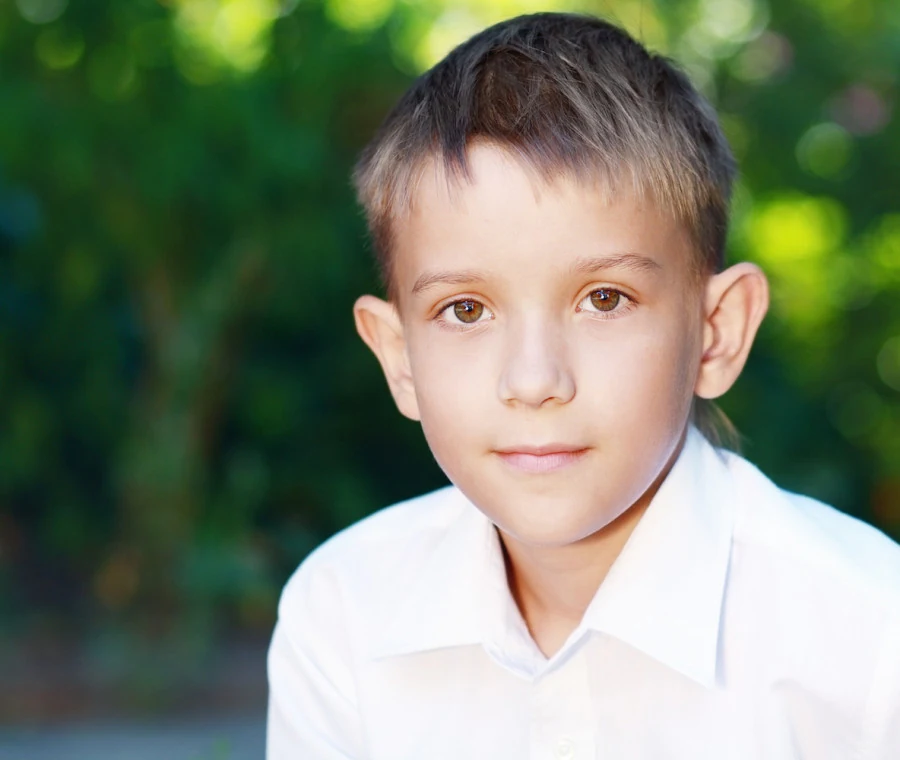
\includegraphics[height=5cm]{Mirko.jpg} & 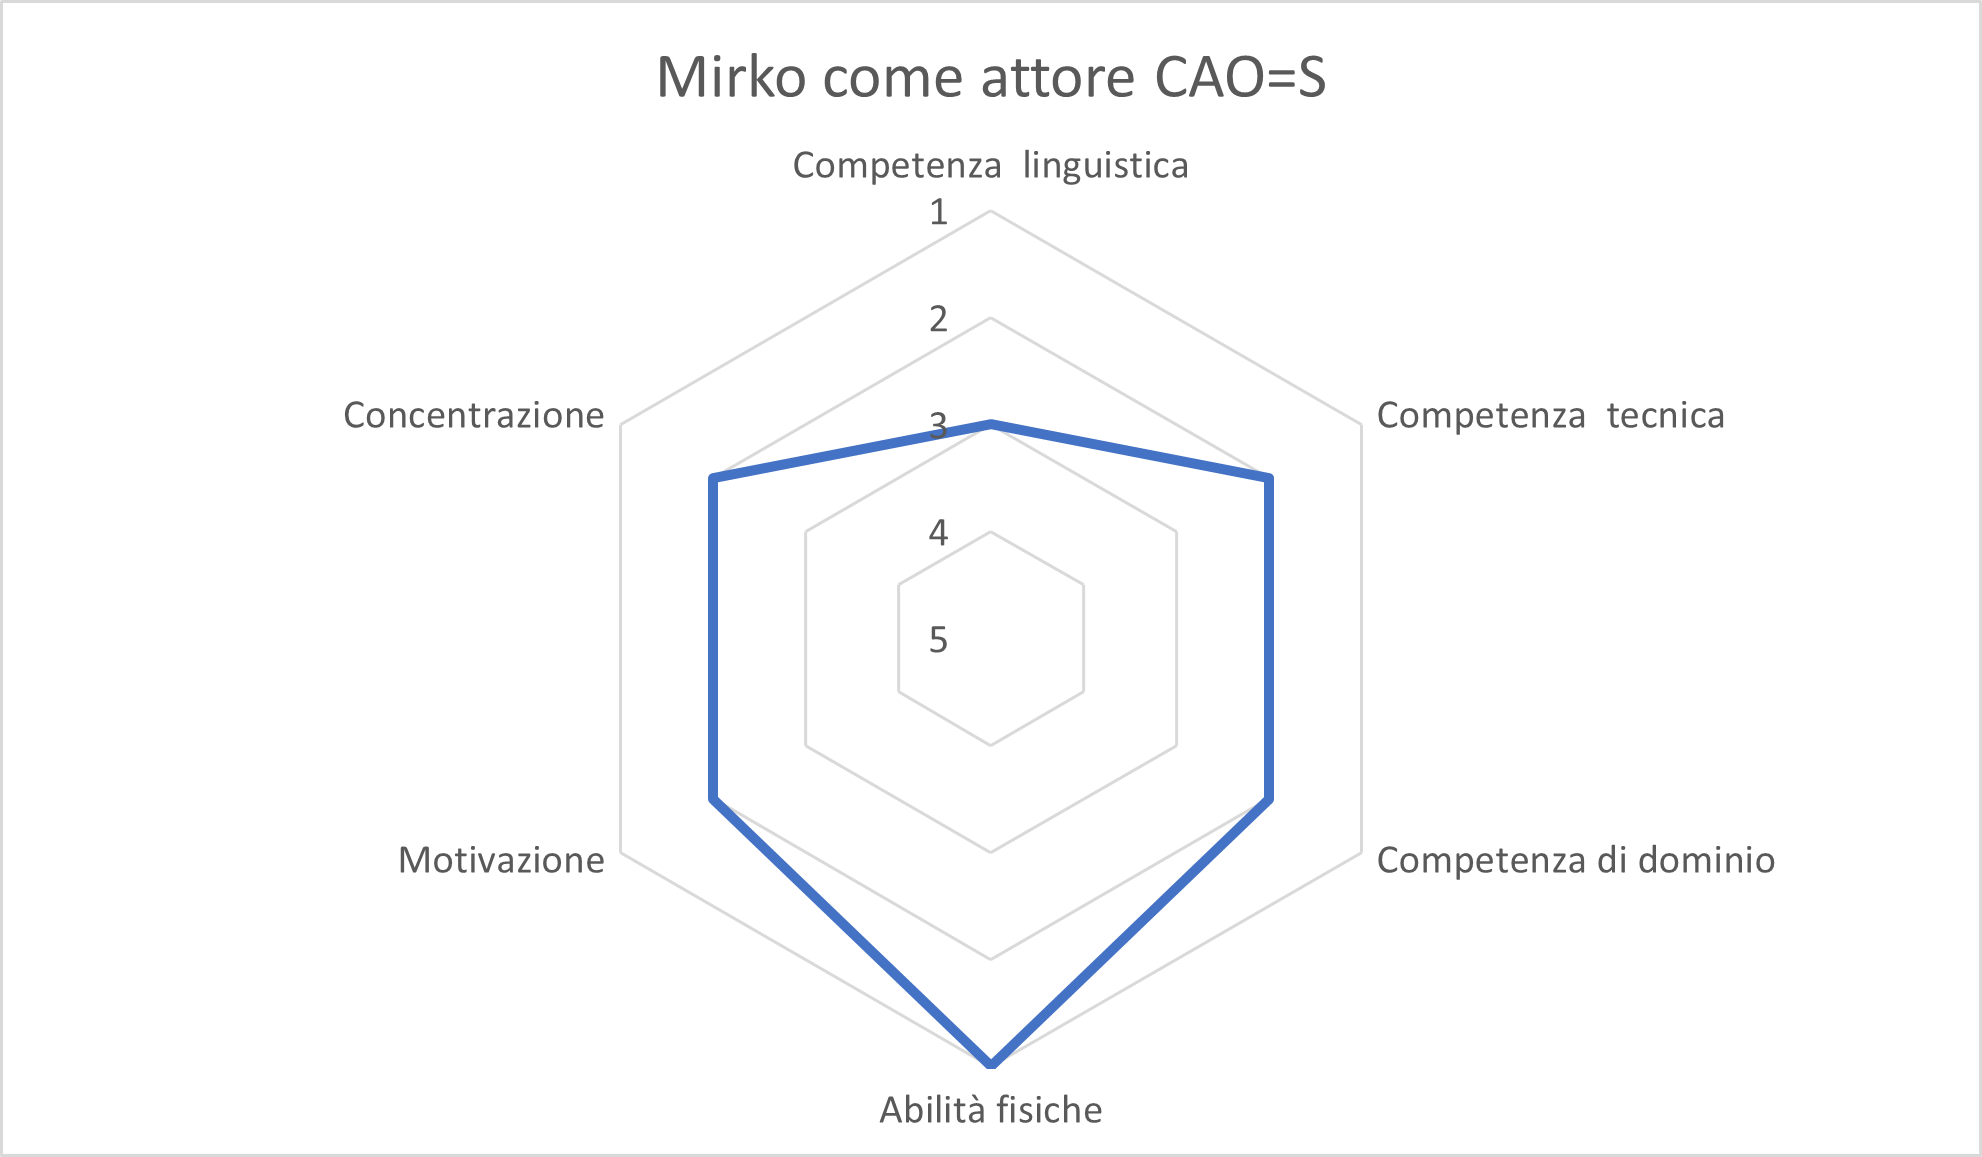
\includegraphics[height=5cm]{MirkoCAOS.png} \\
            \hline
        \end{tabular}
    \end{table}

    \begin{table}[H]
        \begin{tabular}{|c|c|}
            \hline
            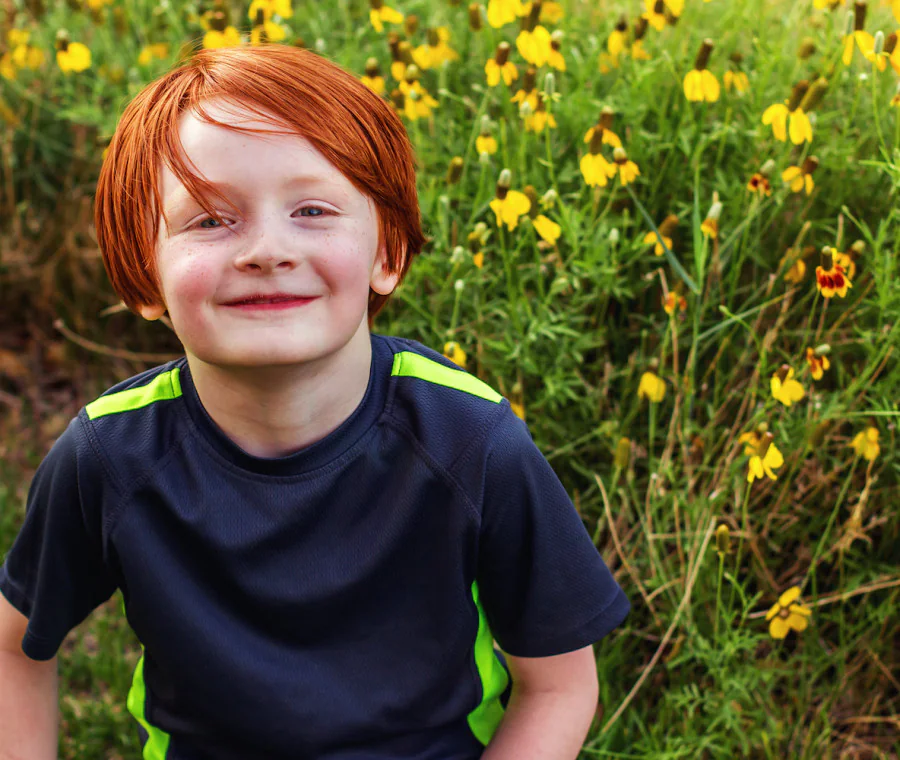
\includegraphics[height=5cm]{Gaetano.jpg} & 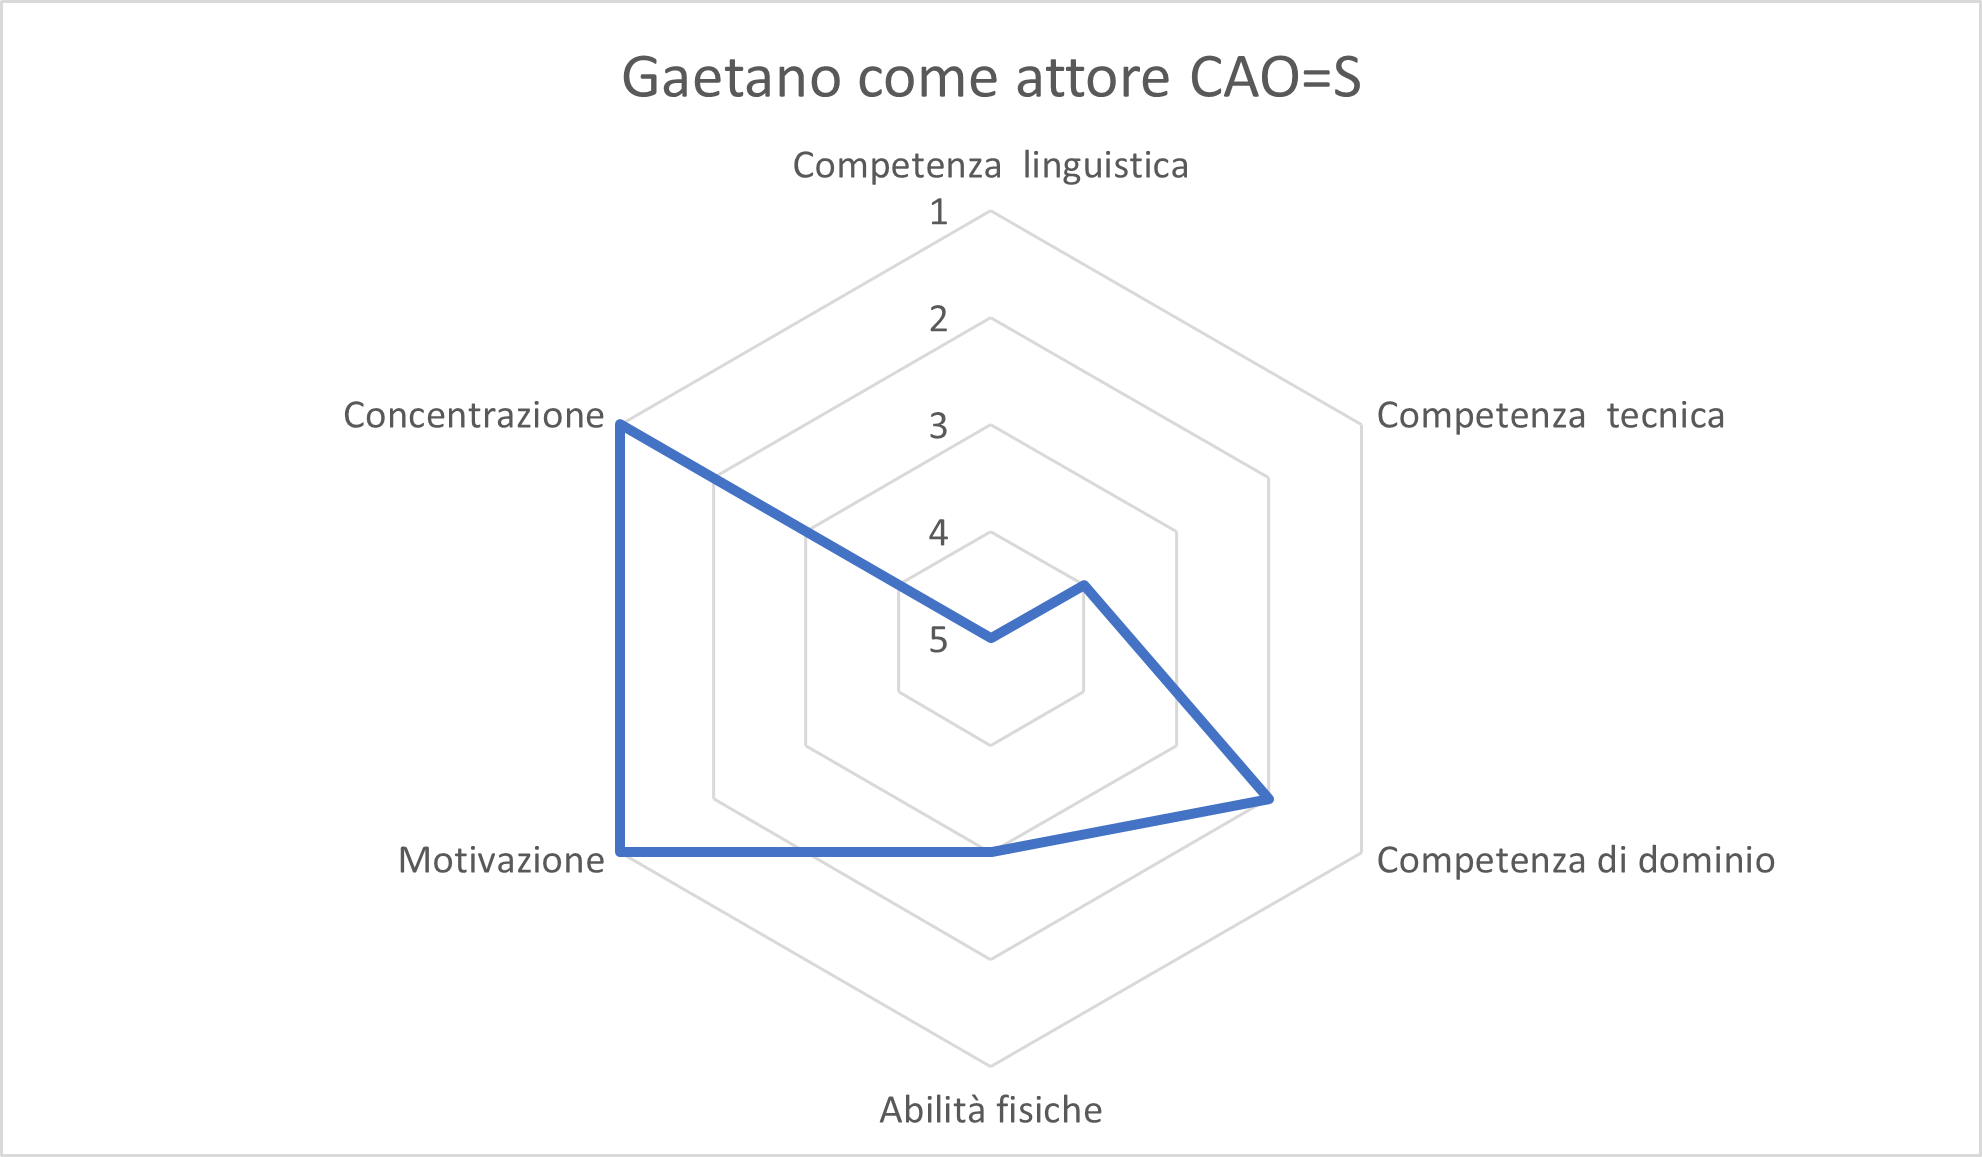
\includegraphics[height=5cm]{GaetanoCAOS.png} \\
            \hline
        \end{tabular}
    \end{table}

    \begin{table}[H]
        \begin{tabular}{|c|c|}
            \hline
            
\includegraphics[height=5cm]{Claudio.jpg} & 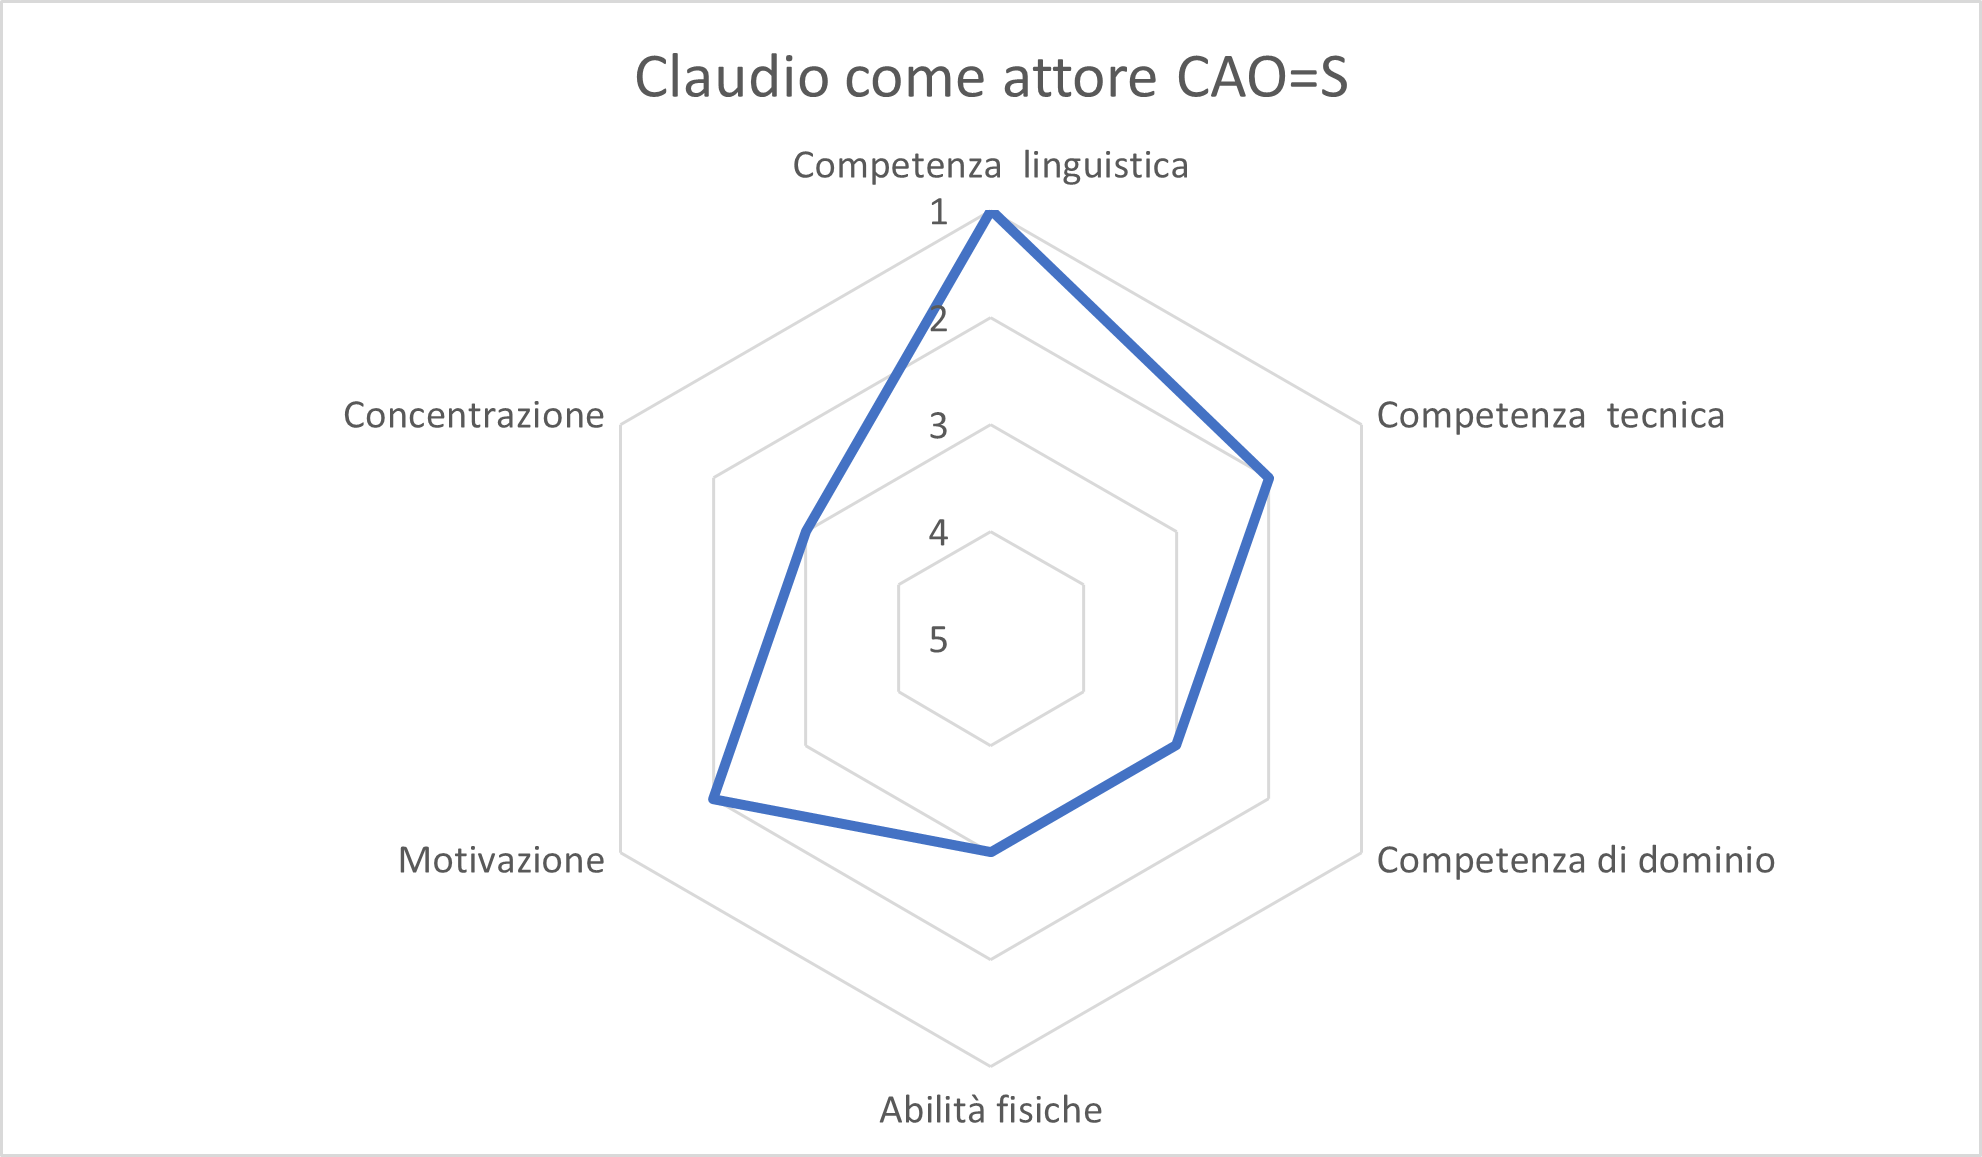
\includegraphics[height=5cm]{ClaudioCAOS.png} \\
            \hline
        \end{tabular}
    \end{table}

    \begin{table}[H]
        \begin{tabular}{|c|c|}
            \hline
            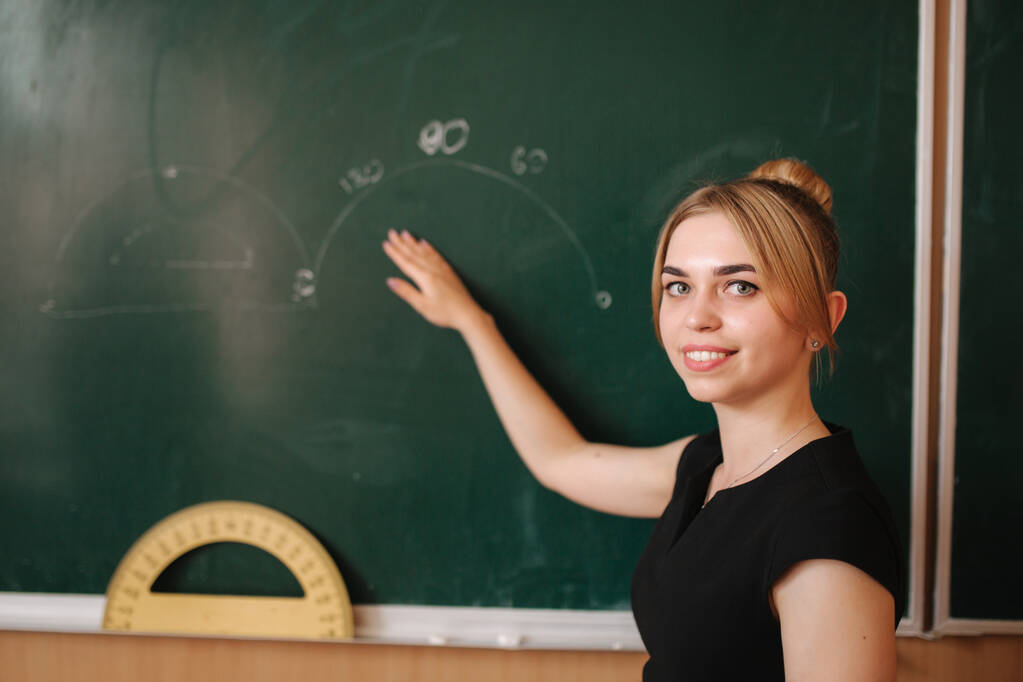
\includegraphics[height=5cm]{Simona.jpg} & 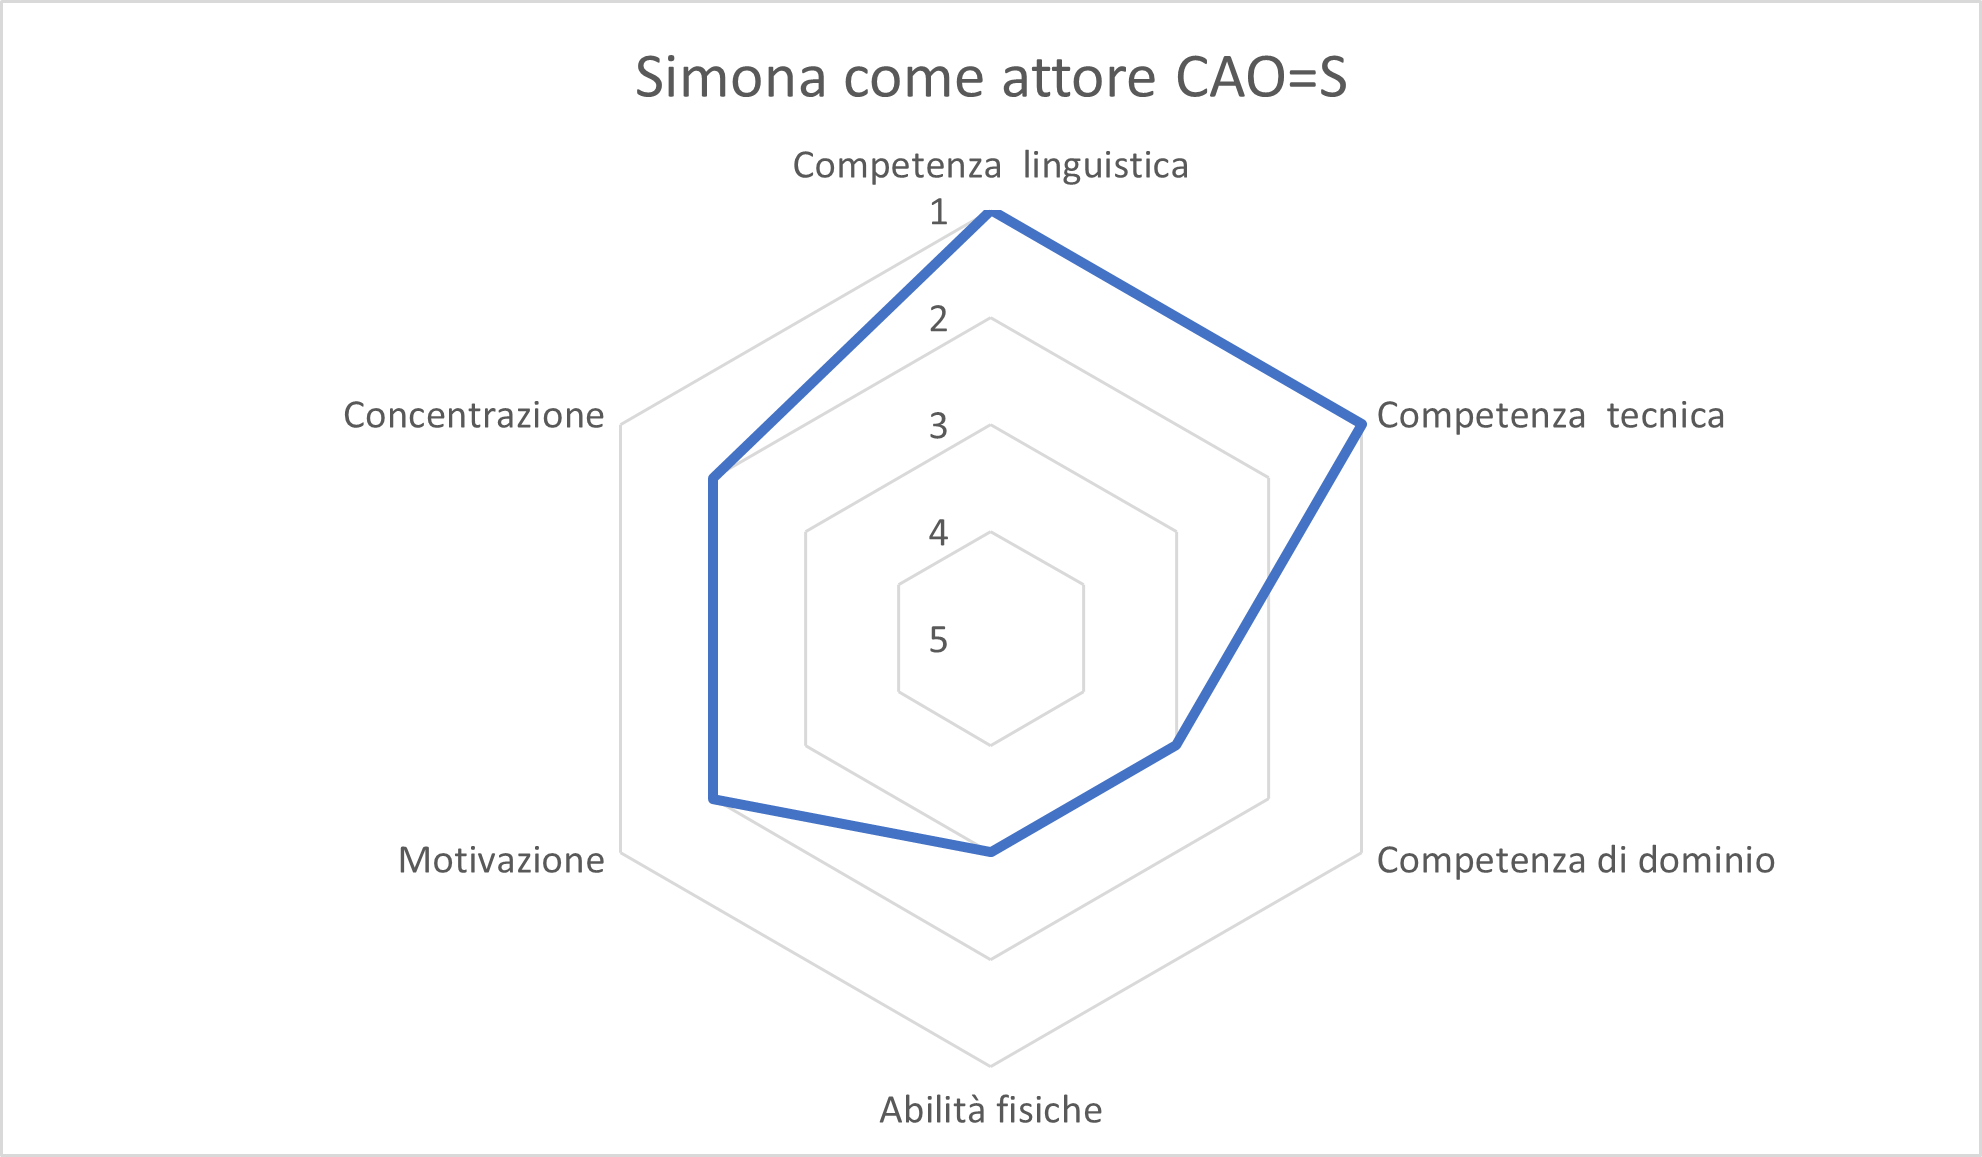
\includegraphics[height=5cm]{SimonaCAOS.png} \\
            \hline
        \end{tabular}
    \end{table}


    \subsection{Operazioni}
    Nel modello CAO=S le operazioni si basano su un modello CRUD, ovvero:
    \begin{itemize}
        \item Create
        \item Read
        \item Update
        \item Delete
    \end{itemize}
    Le singole operazioni compiute dai singoli attori sui singoli concetti vengono inserite in una tabella, che rappresenta, per ciascun attore, i tipi di operazione e i concetti. I nostri attori sono l'utente finale (il giocatore) e il supervisore, quindi dobbiamo fornire due tabelle. La prima è quella del giocatore:

    \begin{table}[H]
        \hspace{-2.5cm}
        \begin{tabular}{|p{2.5cm}|p{3.5cm}|p{3.5cm}|p{3.5cm}|p{3.5cm}|}
            \hline
            \textbf{CONCEPT} & \textbf{CREATE} & \textbf{READ} & \textbf{UPDATE} & \textbf{DELETE} \\
            \hline
            \textbf{Account} & \cellcolor{gray} \textbf{Singola:} Funzionalità di ‘registrarsi come un nuovo utente’ già presente nel sito & \cellcolor{green} \textbf{Individuale completa:} permette di ‘Visualizzare le informazioni relative al proprio account’  & \cellcolor{green} \textbf{Specifico:} Possibilitá di aggiornare il profilo, inserendo l’immagine del profilo e altre informazioni dell’utente stesso & \cellcolor{gray} \textbf{Eliminazione:} Possibilitá di cancellare  l’account giá esistente \\
            \hline
            \textbf{Giochi} & \cellcolor{red} Creazione effettuata dal sito stesso & \cellcolor{green} \textbf{Individuale Completa:} Possibilitá di accedere alla vista completa e giocare nella pagina stessa

            \textbf{Lista Multipla:} In altre sezioni viene mostrata una lista da cui è possibile passare a un individuale completa
             & \cellcolor{red} Aggiornamento effettuato dal sito stesso & \cellcolor{red} Cancellazione effettuata dal sito stesso \\
            \hline
            \textbf{Commento} & \cellcolor{gray} \textbf{Manuale Molteplice:} poiché è possibile effettuare diversi commenti riferiti a uno stesso gioco & \cellcolor{gray} \textbf{Individuale Completa:} Tutte le caratteristiche dei commenti sono visibili & \cellcolor{gray} \textbf{Globale:} Possiede la stessa maschera di visualizzazione & \cellcolor{gray} \textbf{Cancellazione:} il commento viene definitivamente rimosso dalle strutture dati\\
            \hline
            \textbf{Categoria} & \cellcolor{red} Creazione effettuata dal sito stesso & \cellcolor{green} \textbf{Individuale Completa:} Ci sará una pagina dedicata ai giochi di quella determinata categoria

            \textbf{Lista multipla:} è presente una pagina dedicata a tutte le categorie con le relative sottocategorie
            
            \textbf{Individuale Ridotta:} Nel menu è presente una lista di categorie dalle quali è possibile passare a un individuale completa
            
             & \cellcolor{red} Aggiornamento effettuato dal sito stesso & \cellcolor{red} Cancellazione effettuata dal sito stesso \\
            \hline
        \end{tabular}
    \end{table}

    \begin{table}[H]
        \hspace{-2.5cm}
        \begin{tabular}{|p{2.5cm}|p{3.5cm}|p{3.5cm}|p{3.5cm}|p{3.5cm}|}
            \hline
            \textbf{Menu} & \cellcolor{red} Creazione effettuata dal sito stesso & \cellcolor{green} \textbf{Individuale Completa:} Il menu viene visualizzato completamente & \cellcolor{red} Aggiornamento effettuato dal sito stesso & \cellcolor{red} Cancellazione effettuata dal sito stesso \\
            \hline
            \textbf{Filtro} & \cellcolor{red} Creazione effettuata dal sito stesso & \cellcolor{green} \textbf{Ricapitolato Multipla:} Vengono raggruppati tutti i fatti delle istanze dei filtri  & \cellcolor{green} \textbf{Globale:} La vista è la stessa per la selezione dei filtri & \cellcolor{red} \textbf{NO:} non è possibile la cancellazione \\
            \hline
            \textbf{Amici} & \cellcolor{gray} \textbf{Manuale multipla:} Intendiamo l’invio di una (o piú) richiesta di amicizia & \cellcolor{gray} \textbf{Individuale Completa:} Puoi visualizzare il profilo di un amico

            \textbf{Lista Multipla:} poiché puoi visualizzare la lista degli amici
             & \cellcolor{red} \textbf{NO:} non è possibile l’aggiornamento  & \cellcolor{gray} \textbf{Cancellazione:} L’amico viene definitivamente rimosso anche dalle strutture dati\\
            \hline
            \textbf{Descrizione} & \cellcolor{red} Creazione effettuata dal sito stesso & \cellcolor{gray} \textbf{Individuale Completa:} All’intero della pagina del gioco è possibile visionare la descrizione completa & \cellcolor{red} Aggiornamento effettuato dal sito stesso & \cellcolor{red} Cancellazione effettuata dal sito stesso \\
            \hline
            \textbf{Preferiti} & \cellcolor{gray} \textbf{Manuale Multipla:} è possibile mettere nei preferiti uno o piú giochi & \cellcolor{gray} \textbf{Lista Multipla:} poiché puoi visualizzare la lista degli amici preferiti & \cellcolor{red} \textbf{NO:} non è possibile l’aggiornamento & \cellcolor{gray} \textbf{Cancellazione:} La rimozione di un gioco dai preferiti viene definitivamente rimosso anche dalle strutture dati\\
            \hline
            \textbf{FAQ} & \cellcolor{gray} Creazione effettuata dal sito stesso & \cellcolor{green} \textbf{Individuale completa:} Possibilita di leggere l'intera pagina delle FAQ & \cellcolor{red} Aggiornamento effettuato dal sito stesso & \cellcolor{gray} Cancellazione effettuata dal sito stesso \\
            \hline
            \textbf{Parental Control} & \cellcolor{red} \textbf{NO:} non è possibile creare & \cellcolor{red} \textbf{NO:} Non è possibile visualizzare, è possibile visualizzare solo dall’utente supervisore & \cellcolor{red} \textbf{NO:} non è possibile l’aggiornamento & \cellcolor{red} \textbf{NO:} non è possibile la cancellazione \\
            \hline
        \end{tabular}
        \caption{\label{tab:giocatore}Tabella del giocatore}
    \end{table}



    Di seguito mostriamo la tabella del supervisore, fondamentalmente identica alla precedente con la sola differenza nel concetto del Parental Control:

    \begin{table}[H]
        \hspace{-2.5cm}
        \begin{tabular}{|p{2.5cm}|p{3.5cm}|p{3.5cm}|p{3.5cm}|p{3.5cm}|}
            \hline
            \textbf{CONCEPT} & \textbf{CREATE} & \textbf{READ} & \textbf{UPDATE} & \textbf{DELETE} \\
            \hline
            ... & ... & ... & ... & ... \\
            \hline
            \textbf{Parental Control} & \cellcolor{green} \textbf{Manuale Singola:} è possibile creare uno e un solo parental control & \cellcolor{green} \textbf{Individuale Completa:} Possibilitá di vedere tutte le caratteristiche del parental control & \cellcolor{green} \textbf{Globale:} Possiede la stessa maschera della creazione & \cellcolor{green} \textbf{Cancellazione:} Rimozione del parental control anche dalle strutture dati \\
            \hline
        \end{tabular}
        \caption{\label{tab:supervisore}Tabella del supervisore}
    \end{table}
    
    \subsubsection{Note}
    In questa prospettiva, creare significa che l’utente, attraverso il sito, crea un qualcosa di nuovo (come un account o un commento), lo stesso vale per l’aggiornamento e l’eliminazione. La voce “Read” sta ad indicare tutto ciò che l’utente può osservare di quel determinato concetto e il tipo di vista che l'utente ha su quel concetto. In rosso vengono messe tutte quelle operazioni che vengono eseguite da Gioco.it e l’utente non può intervenire in alcun modo. In grigio tutte le operazioni già presenti nel sito, che non hanno subito modifiche dopo la nostra progettazione. In verde le nostre modifiche apportate al sito.

    \section{Progettazione dell'interazione}
    In questa sezione definiremo l'architettura dell'informazione che abbiamo definito nella sezione \ref{section:architettura dell'informazione} e nelle viste CAO=S (sezione \ref{section:CAOS}), prima proponendo dei Blueprints, uno schema in cui viene spiegato il modello concettuale del sito, e successivamente proporremo i Wireframes, delle rappresentazioni delle schermate principali del sito.

    \subsection{Homepage}
    La homepage dovrà essere più coerente e ordinata rispetto all'attuale design, più orientato alla minimizzazione del carico cognitivo dell'utente. Il nuovo design dovrà permettere sia di trovare giochi nuovi e sia di presentare giochi utilizzati di frequente. Inoltre, essa dovrà mostrare tutte le funzionalità messe a disposizione del sito (es: categorie, account, ecc).

    \subsubsection{Header}
    Essa permetterà di ricercare i giochi per nome, visualizzare le categorie, visualizzare il proprio account e avrà il logo per tornare alla homepage. A differenza del vecchio design permetterà di visualizzare tutte le categorie e non soltanto alcune. 

    \subsubsection{Footer}
    Esso conterrà le informazioni dell'azienda, assistenza clienti (FAQ) e la possibilità di cambiare la lingua. Il design rimarrà pressoché lo stesso.
    
    \subsection{Card del gioco}
    Nella versione attuale le card dei giochi non contengono informazione rilevanti per i supervisori, infatti nel nuovo design saranno presenti dei simboli che descrivono i contenuti del gioco (es: limiti di età, violenza, presenza di armi, ecc).

    \subsection{Gioco}
    La schermata del gioco dovrà contenere gli stessi elementi che contiene attualmente. Sarà necessario quindi un riquadro per la visualizzazione del gioco e la sua descrizione. Saranno presenti i comandi che permettono di andare direttamente a mettere nei preferiti un gioco e a spostarsi nella sezione commenti. Poichè come detto nella sezione di Inspezione \ref{} è presente dell'inutile spazio vuoto alla destra dei giochi il nostro redesign andrà ad occupare lo spazio lasciato vuoto, riempiendolo per quanto possibile con la schermata di gioco. Sarà anche importante mantenere la sezione legata al supporto e alla spiegazione del gioco (precedentemente erroneamente chiamata "Soluzione").

    \subsection{Account}
    \subsubsection{Login \& Registrazione}
    Come detto in precedenza la schermata di login \& registrazione non ha particolari problemi, il suo design resterà pressoché invariato. 
    %TODO: Mettere password supervisore
    \subsubsection{Conversazioni}
    La sezione conversazioni andrà profondamente rivista rispetto al suo attuale funzionamento, cioè quello di una chat pubblica sul profilo di un utente. Abbimo deciso di riordinare questa sezione e di renderla un mini-forum in cui un utente può creare delle discussioni con un titolo a cui tutti gli utenti (o anche solo gli utenti amici) possono rispondere. Pensiamo a questa sezione come un modo per gli utente di discutere, scambiarsi idee e risultati a proposito dei giochi che loro giocano, separata dalla sezione commenti dei giochi proprio per la possibilità di far parlare tra di loro utenti amici. 
    \subsubsection{Giochi preferiti}
    La sezione dei giochi preferiti conterrà la lista di giochi che l'utente ha selezionato come preferiti. Come attualmente è già presente sul sito, puntando un gioco con il mouse ci saranno due possibilità: giocare al gioco o eliminarlo dalla lista dei preferiti. Non prevediamo quindi grandi cambiamenti a questa sezione.
    \subsubsection{Amici}
    Anche per la sezione amici non prevediamo grandi stravolgimenti. Sarà quindi possibile inviare richieste di amicizia, vedere la lista di amici, eliminare un amico e vedere quelle che sono le richieste di amicizia in arrivo. 
    \subsubsection{Impostazioni}
    In questa sezione il nostro principale lavoro sarà quello di andare a permettere la modifica del nome utente, delle mail e della password (l'unica cosa modificabile attualmente). Inoltre, oltre alle funzionalità già presenti ci sarà un rimando alla funzione "Parental Control".
    \subsubsection{Parental control}
    Questa sezione del sito sarà una nuova aggiunta e permetterà ai soli utenti supervisori di applicare limiti all'utilizzo del sito. Sarà quindi necessaria una password per l'accesso. In particolare sarà possibile in questa sezione del sito applicare un limite di tempo d'uso per il sito, oltre che applicare una serie di filtri. Sarà possibile infatti:
    \begin{itemize}
        \item applicare una limitazione di tempo d'uso 
        \item nascondere i giochi che superano una determinata età
        \item nascondere i giochi che presentano determinate caratteristiche (es. presenza di armi, violenza, mostri)
        \item selezionare sono alcune caratteristiche di giochi (es. giochi logici o matematici)
    \end{itemize}
    
    \section{Blueprints}
    All'interno dei Blueprint distinguiamo come mostrato nella legenda sottostante le pagine, i componenti e le parti che andremo a definire in un blueprint in una fase successiva.
    \begin{figure}[H]
        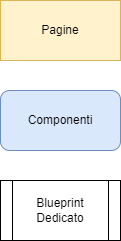
\includegraphics[height=5cm]{Legenda.png}
        \centering
    \end{figure}

    Partendo da ció, partiamo dalla Home Page distinguendo se é l'utente ha eseguito il login o meno.
    Illustriamo cosi, tutte le sue componenti ed espandiamo successivamente le pagine più importanti.

    \begin{figure}[H]
        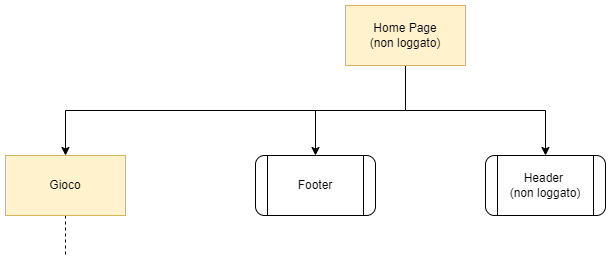
\includegraphics[width=\linewidth]{BP_homepage non loggato.png}
        \centering
        \caption{Blueprint Homepage: Utente non loggato}
    \end{figure}

    L'\textbf{Header} invece avrá la struttura seguente:
    
    \begin{figure}[H]
        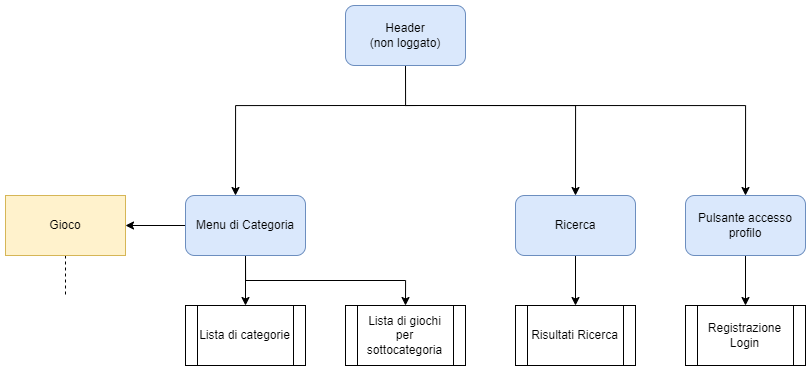
\includegraphics[width=\linewidth]{BP_HeaderNOLOG.png}
        \centering
        \caption{Blueprint Header: Utente non loggato}
    \end{figure}


    Nel caso l'utente effettui il login terremo in considerazione il seguente Blueprint:

    \begin{figure}[H]
        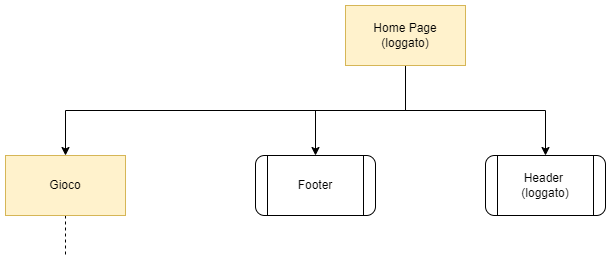
\includegraphics[width=\linewidth]{BP_homepage loggato.png}
        \centering
        \caption{Blueprint Homepage: Utente loggato}
    \end{figure}


    Andremo ad espandere successivamente l'\textbf{Header} della pagina come segue:

    \begin{figure}[H]
        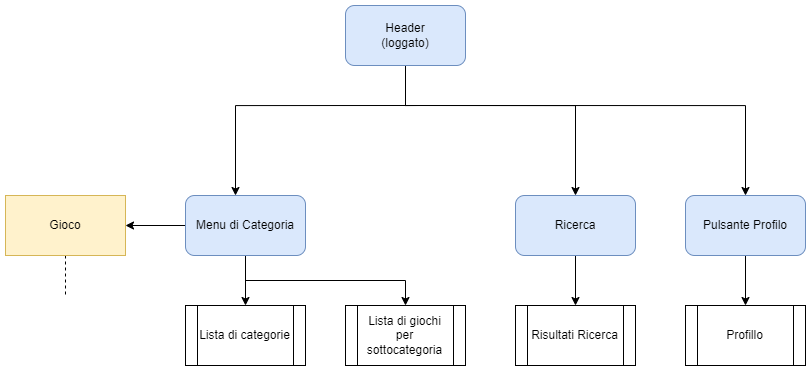
\includegraphics[width=\linewidth]{BP_HeaderLog.png}
        \centering
        \caption{Blueprint Header: Utente loggato}
    \end{figure}

    Nell'Header troviamo componenti quali: la ricerca, il pulsante che ti permette di accedere al profilo(poiché ricordiamo che l'utente ha eseguito l'accesso), il menu contenente tutte le categorie e che possono riferirsi direttamente a una pagina contenente il \textbf{Gioco}.\\

    Per eseguire l'accesso é necessario passare attraverso un meccanismo di login/registrano illustrato come segue, che al termine in caso di successo verrá reindirizzato alla HomePage (loggato):

    \begin{figure}[H]
        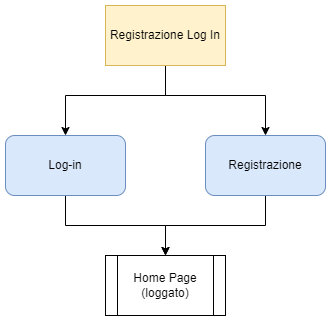
\includegraphics[width=.6\linewidth]{BP_registrazione login.png}
        \centering
        \caption{Blueprint Login/Registrazione}
    \end{figure}

    Espandiamo ora il \textbf{Footer} che contiene la pagina relativa alle FAQ e alle informazioni della azienda; inoltre un componente che ti permette di cambiare la lingua del sito e ti reindirizza alla homepage con la lingua modificata.
    \begin{figure}[H]
        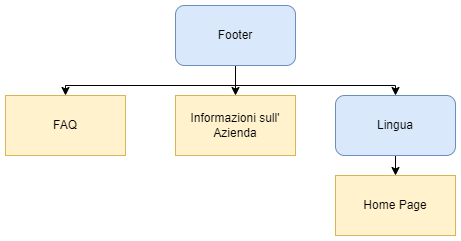
\includegraphics[width=.8\linewidth]{BP_footer.png}
        \centering
        \caption{Blueprint Footer}
    \end{figure}

    Nell'\textbf{Header} troviamo lo strumento per effettuare una ricerca che mostrerá come risultati una lista di giochi ai quali é possibile accedere.
    \begin{figure}[H]
        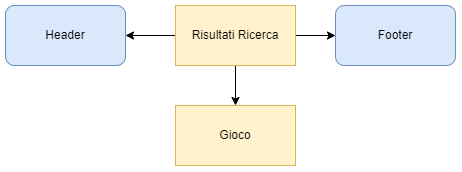
\includegraphics[width=.8\linewidth]{BP_RisultatiRicerca.png}
        \centering
        \caption{Blueprint Risultati Ricerca}
    \end{figure}

    Troviamo sempre nell'Header 
    La pagina dei \textbf{Giochi} conterrá oltre la possibilitá di giocare anche una descrizione e una sezione commenti in cui tutti gli utenti possono discuterlo.
    Il componente spiegazione é solitamente un video-tutorial del gioco.
    \begin{figure}[H]
        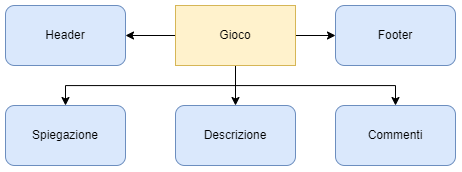
\includegraphics[width=\linewidth]{BP_Gioco.png}
        \centering
        \caption{Blueprint Gioco}
    \end{figure}

    L'\textbf{Area Riservata} riferito al profilo dell'utente contiene oltre all'Header e Footer, componenti quali la lista dei preferiti, degli amici e una sezione dedicata alle conversazioni. 
    É possibile inoltre accedere alle pagine delle impostazione, del parental control e alla modifica dell'immagine del profilo. 
    \begin{figure}[H]
        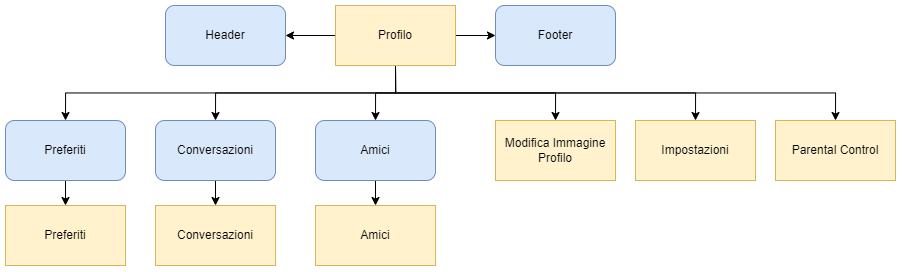
\includegraphics[width=\linewidth]{BP_profilo.png}
        \centering
        \caption{Blueprint Area Riservata}
    \end{figure}


    É Possibile accedere a una pagina relativa alle lista di categorie, che conterra sempre Header e Footer, dalla quale é possibile accedere ad un'ulteriore pagina relativa ad una determinata sottocategoria.
    \begin{figure}[H]
        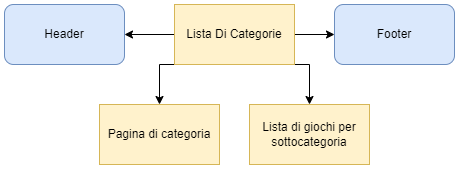
\includegraphics[width=.7\linewidth]{BP_listaCategoria.png}
        \centering
        \caption{Blueprint Lista di Categoria}
    \end{figure}
    Queste sottocategorie conterranno una lista di giochi appartenenti a quella determinata classe.
    \begin{figure}[H]
        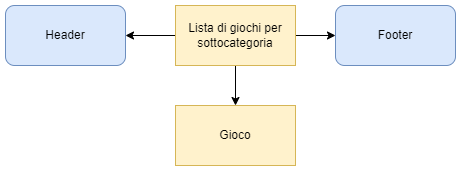
\includegraphics[width=.7\linewidth]{BP_ListaGiochiPerSottocategoria.png}
        \centering
        \caption{Blueprint Lista di giochi per sottocategoria}
    \end{figure}

    \section{Wireframes}
    Illustriamo qui di seguito i Wireframes delle schermate principali

    \subsection{Homepage}
    Dopo le nostre modifiche l'Homepage si presenterá cosi:

    \begin{figure}[H]
        \centering
        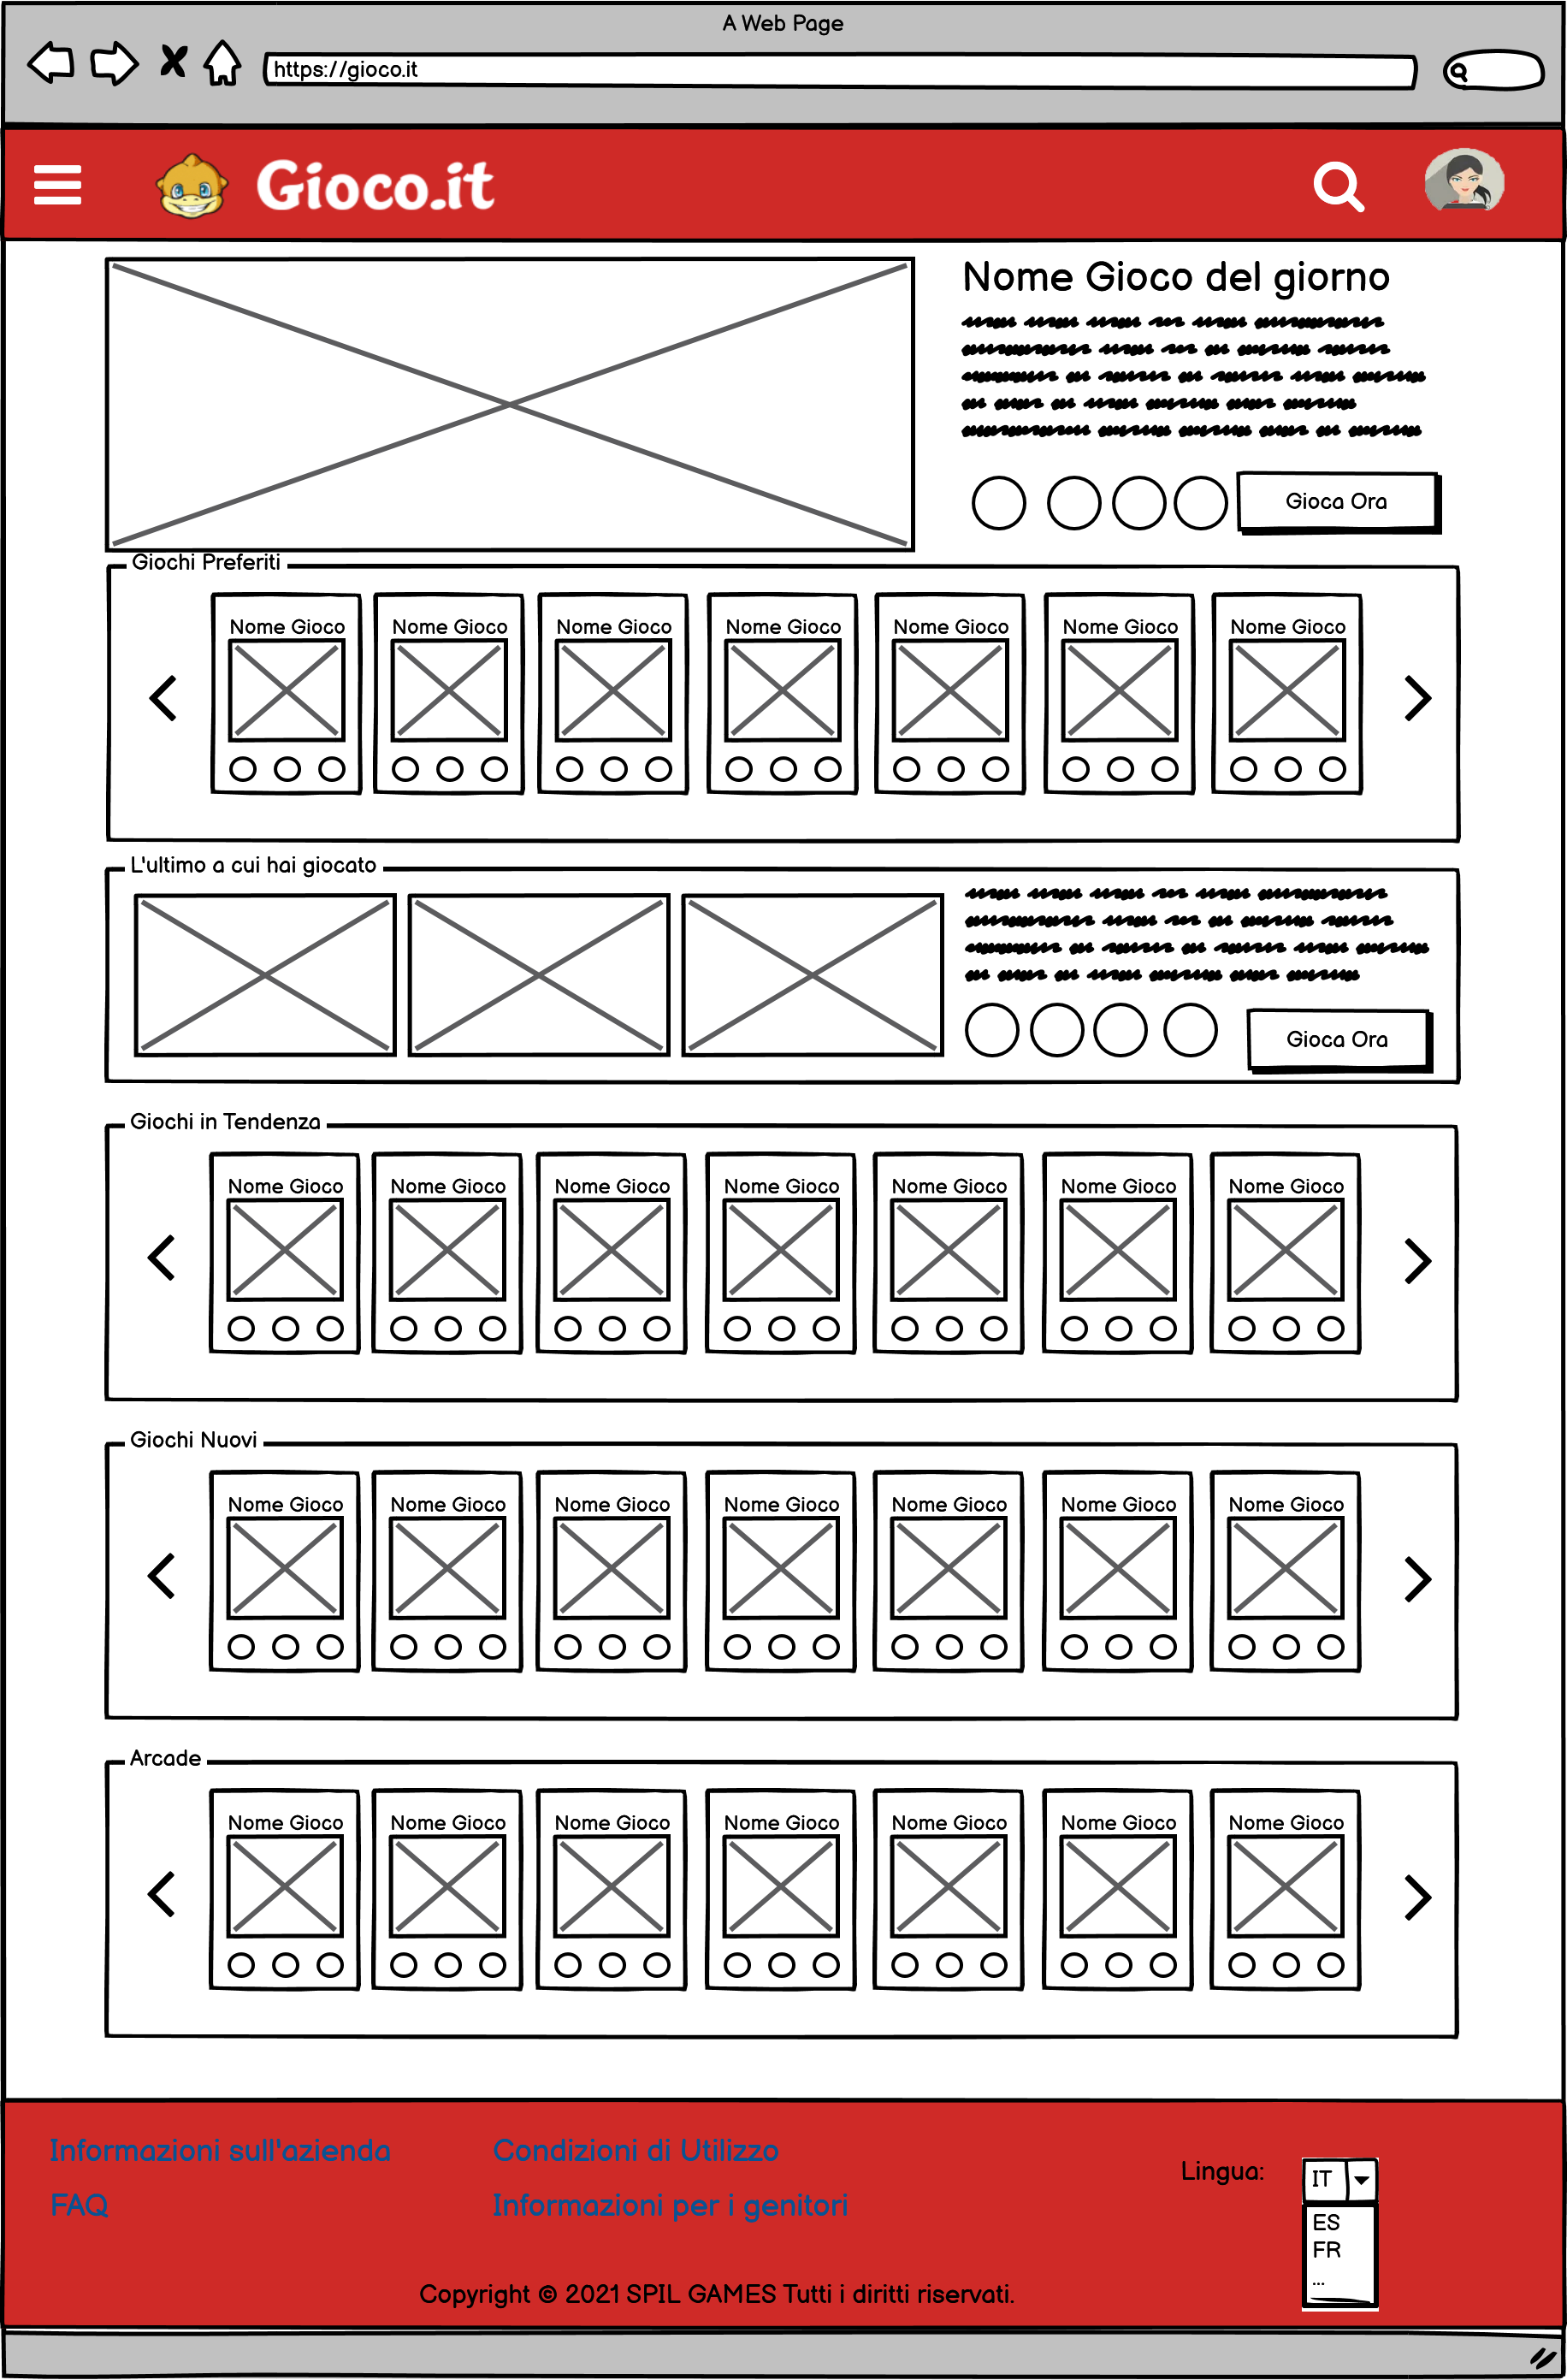
\includegraphics[width=\linewidth]{WHomepage.png}
        \caption{Wireframes per HomePage}
    \end{figure}

         L'\textbf{Header} é stato modificato rendendolo piú semplice e minimale. Il menú é stato totalmente rimpiazzato dalla Toast Icon, il pannello di ricerca verrá mostrato solo al click nell'apposita icona\\
         
         Il \textbf{Footer} contiene gli stessi collegamenti contenuti in precedenza e viene ridotto lo spazio occupato dalla funzionalità del cambio della lingua\\


         Per quanto riguardo il \textbf{Corpo} della homepage  é stato modificato il design della pagina dalla griglia in cui si presentava in precedenza, ad una versione organizzata in liste.
         Inoltre é stata aggiunta una sezione \textbf{in primo piano} che contiente il 'Gioco del giorno' che coglierá subito il colpo d'occhio dell'utente.
         La Homepage inoltre presenterá due diversificazioni in caso l'utente abbia giá eseguito l'accesso o meno(nella figura a fianco come vediamo in alto l'utente é gia loggato).
         In caso sia loggato verrá mostrato una sezione contente i suoi giochi preferiti e l'ultimo gioco a cui ha giocato; in caso contrario queste saranno sostituite da altre categorie presenti nel sito stesso.
         Per ogni gioco troviamo sotto le immagini delle icone che forniscono informazioni sulla tipologia di gioco e sui suoi contenuti (generalmente utile ai supervisori e ai genitori).
         

    \subsection{Barra di Ricerca}
    \begin{figure}[H]
        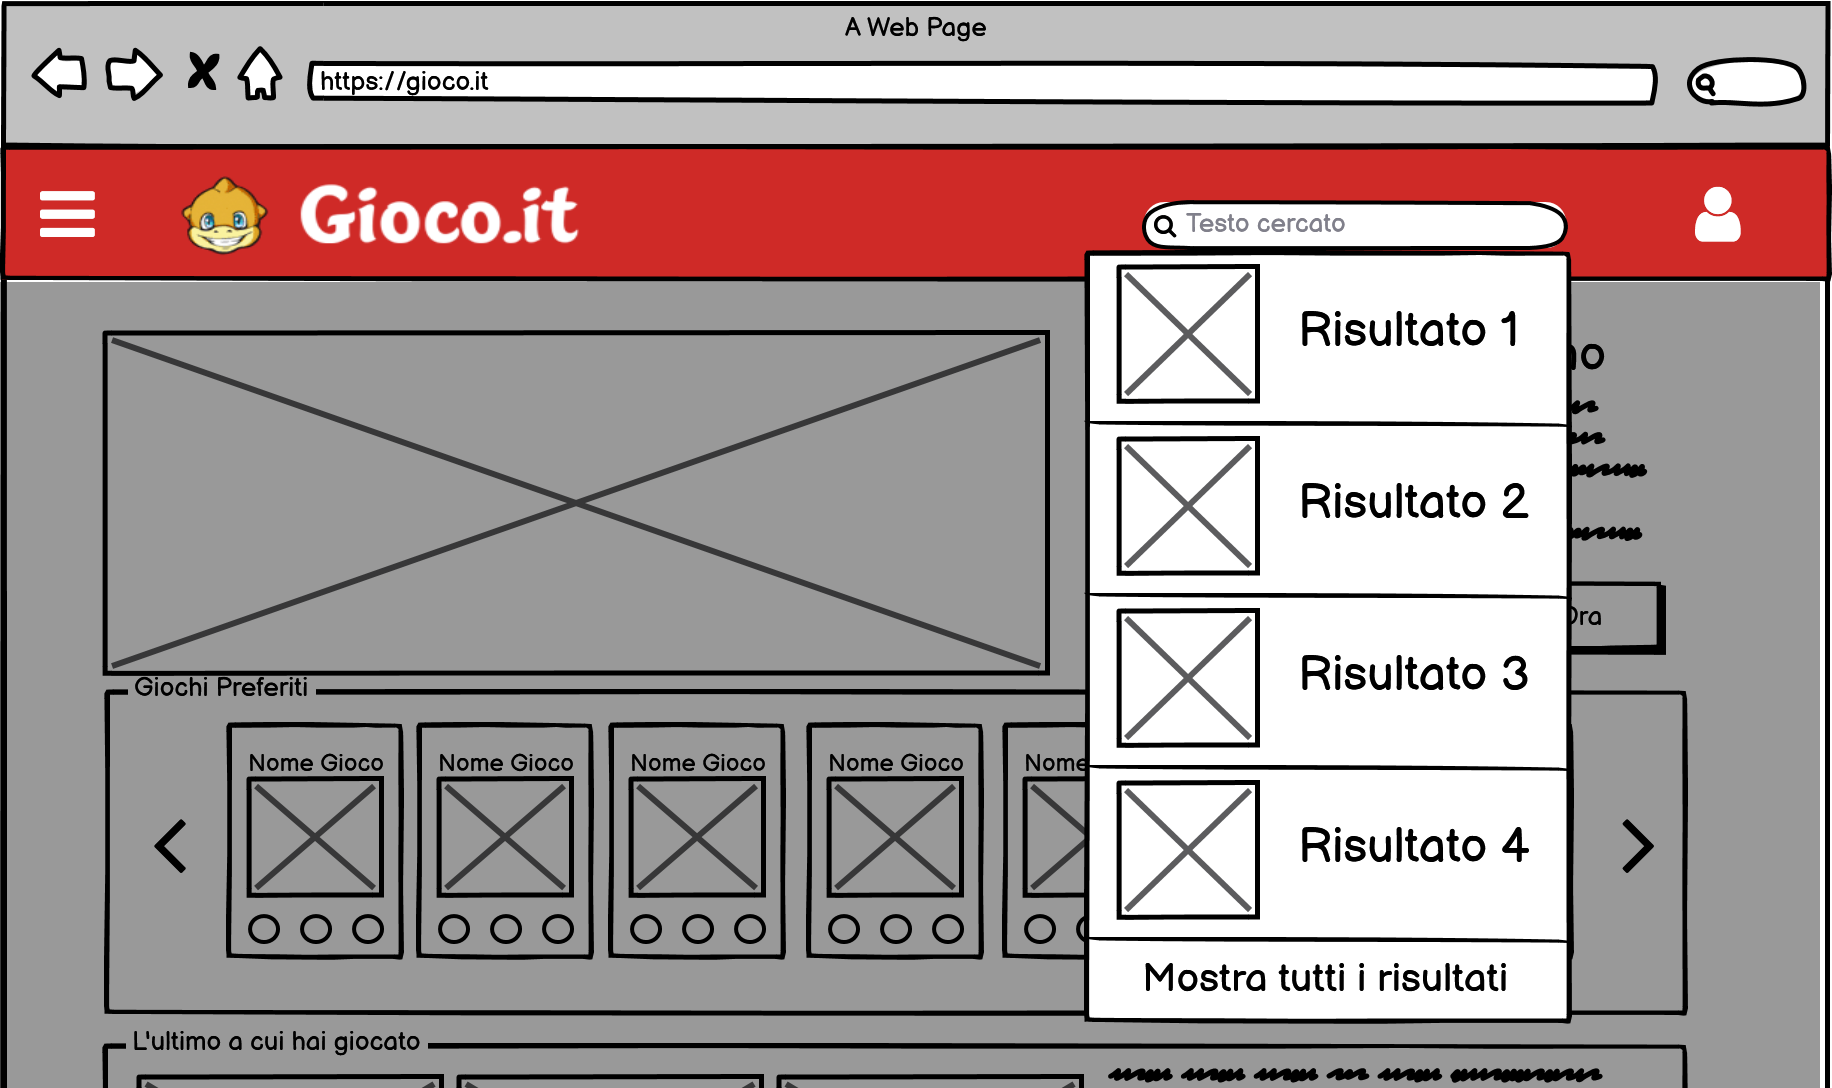
\includegraphics[width=\linewidth]{WSearchBar.png}
        \centering
    \end{figure}
    
    Al click dell'icona della ricerca si aprirá un campo di testo nel quali si potrá digitare la ricerca.
    Durante la digitazione verranno mostrati i risultati piu pertinenti rispetto a quella ricerca, in caso non fossero sufficienti il bottone 'Mostra altri risultati' reindirizzerá alla pagina contenti tutti i risultati di quella ricerca(Vedi Wireframe Successivo)

    \begin{figure}[H]
        \hspace{-1.5cm}
        \begin{minipage}[b]{8cm}
            \centering
            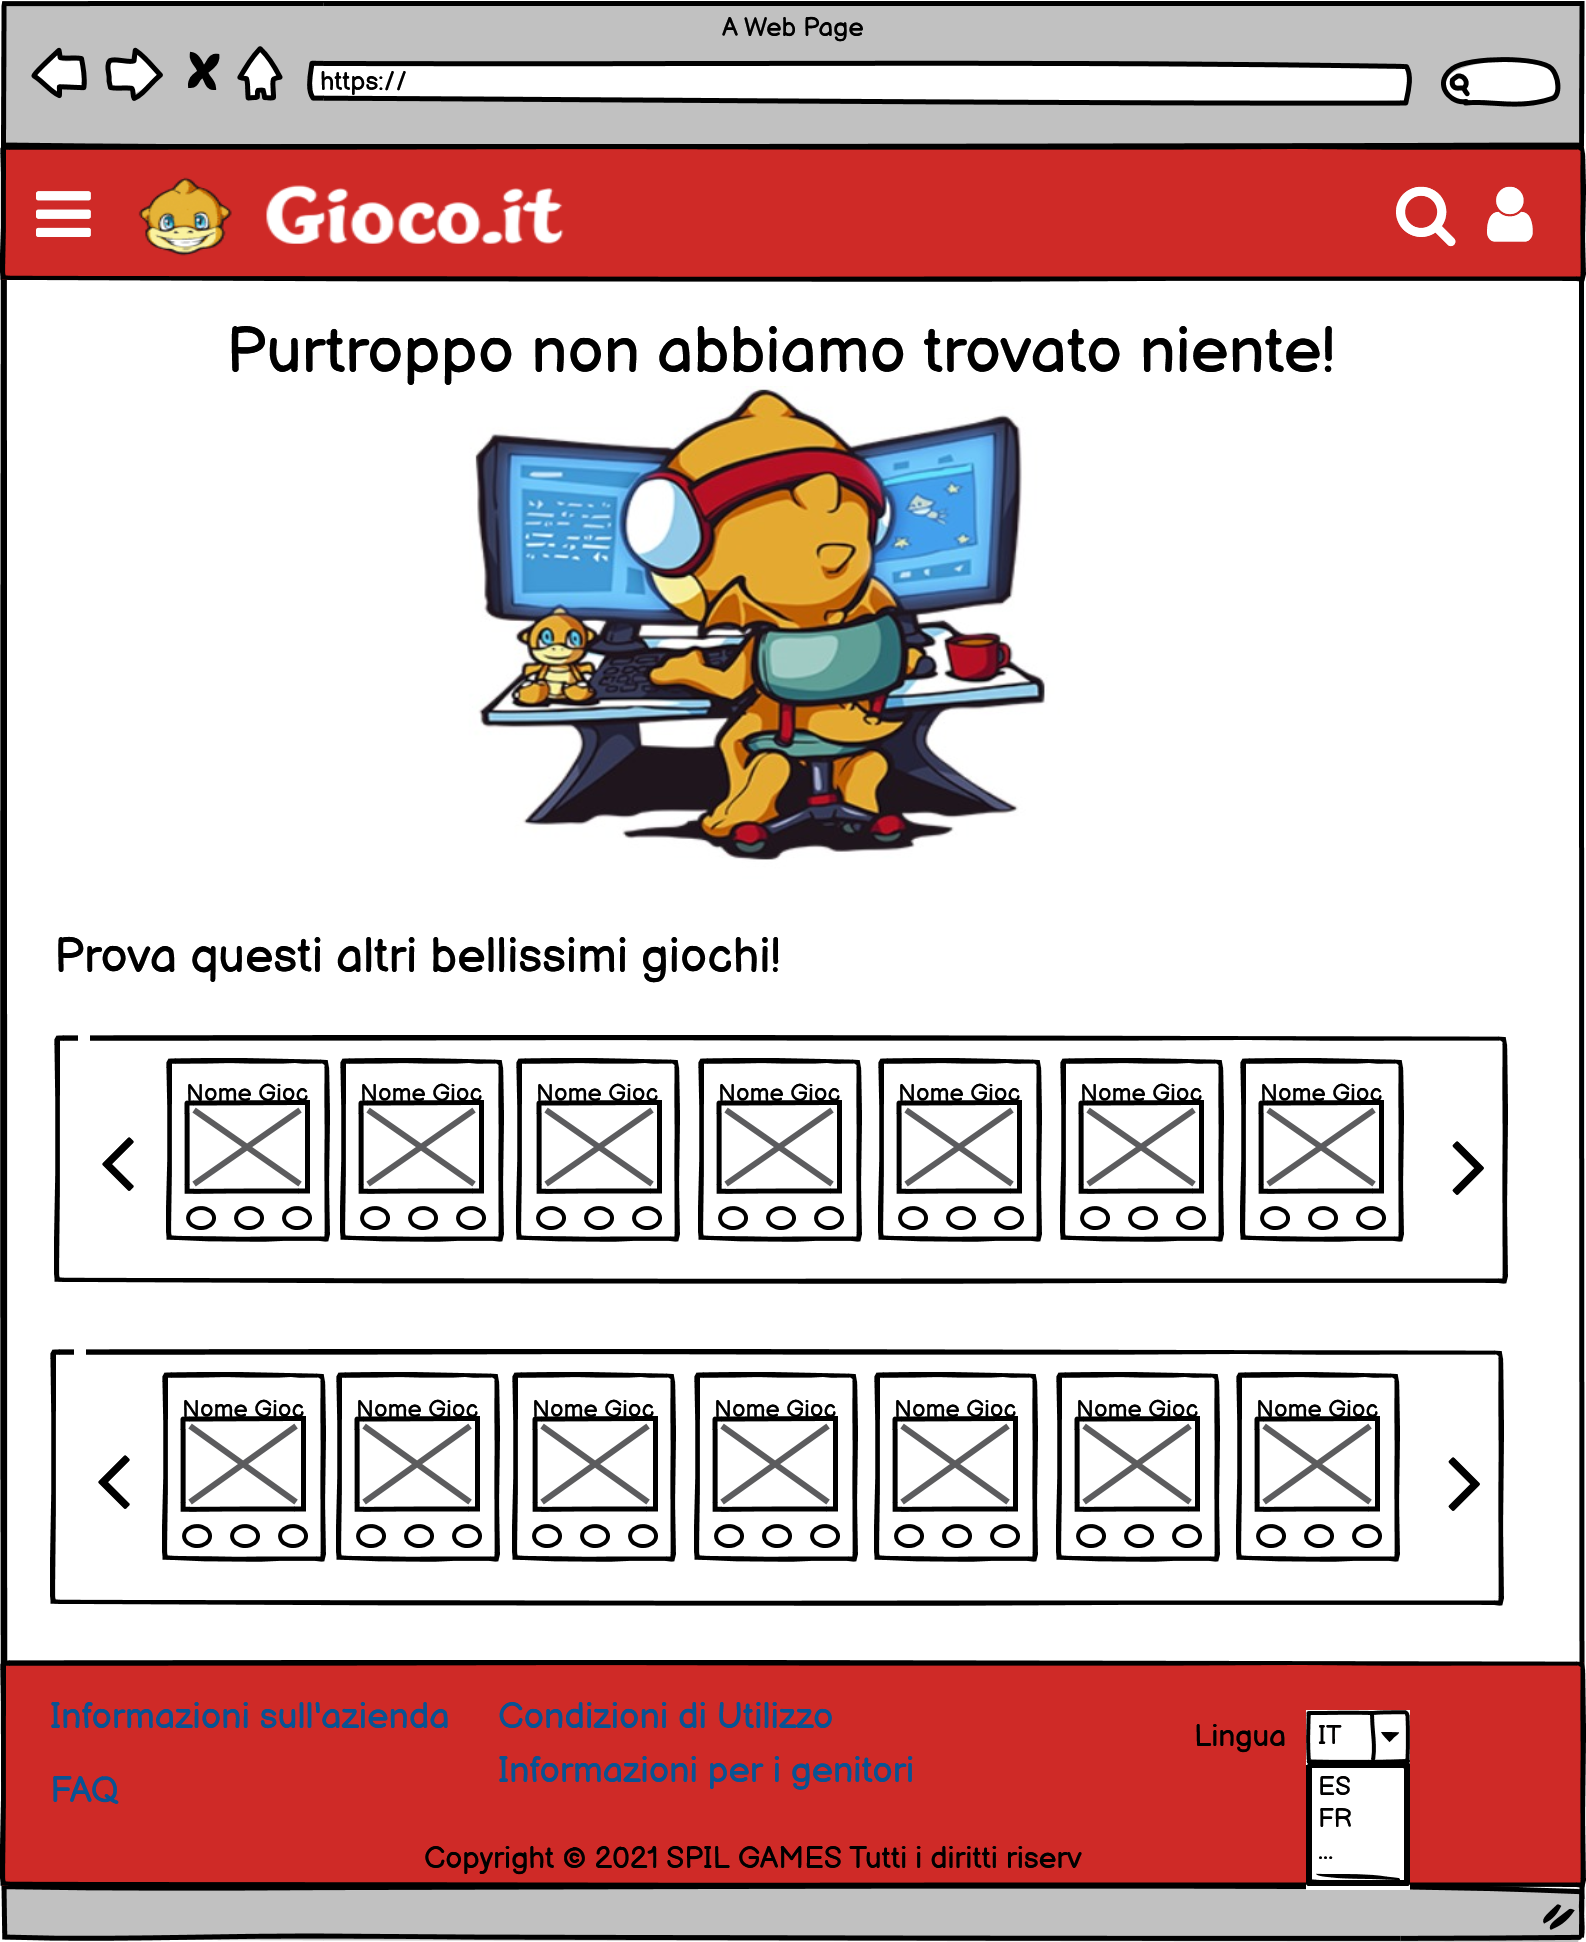
\includegraphics[width=8cm]{WEmpySearchResult.png}
            \end{minipage}
            \ \hspace{2mm} \hspace{3mm} \
            \begin{minipage}[b]{8cm}
            \centering
            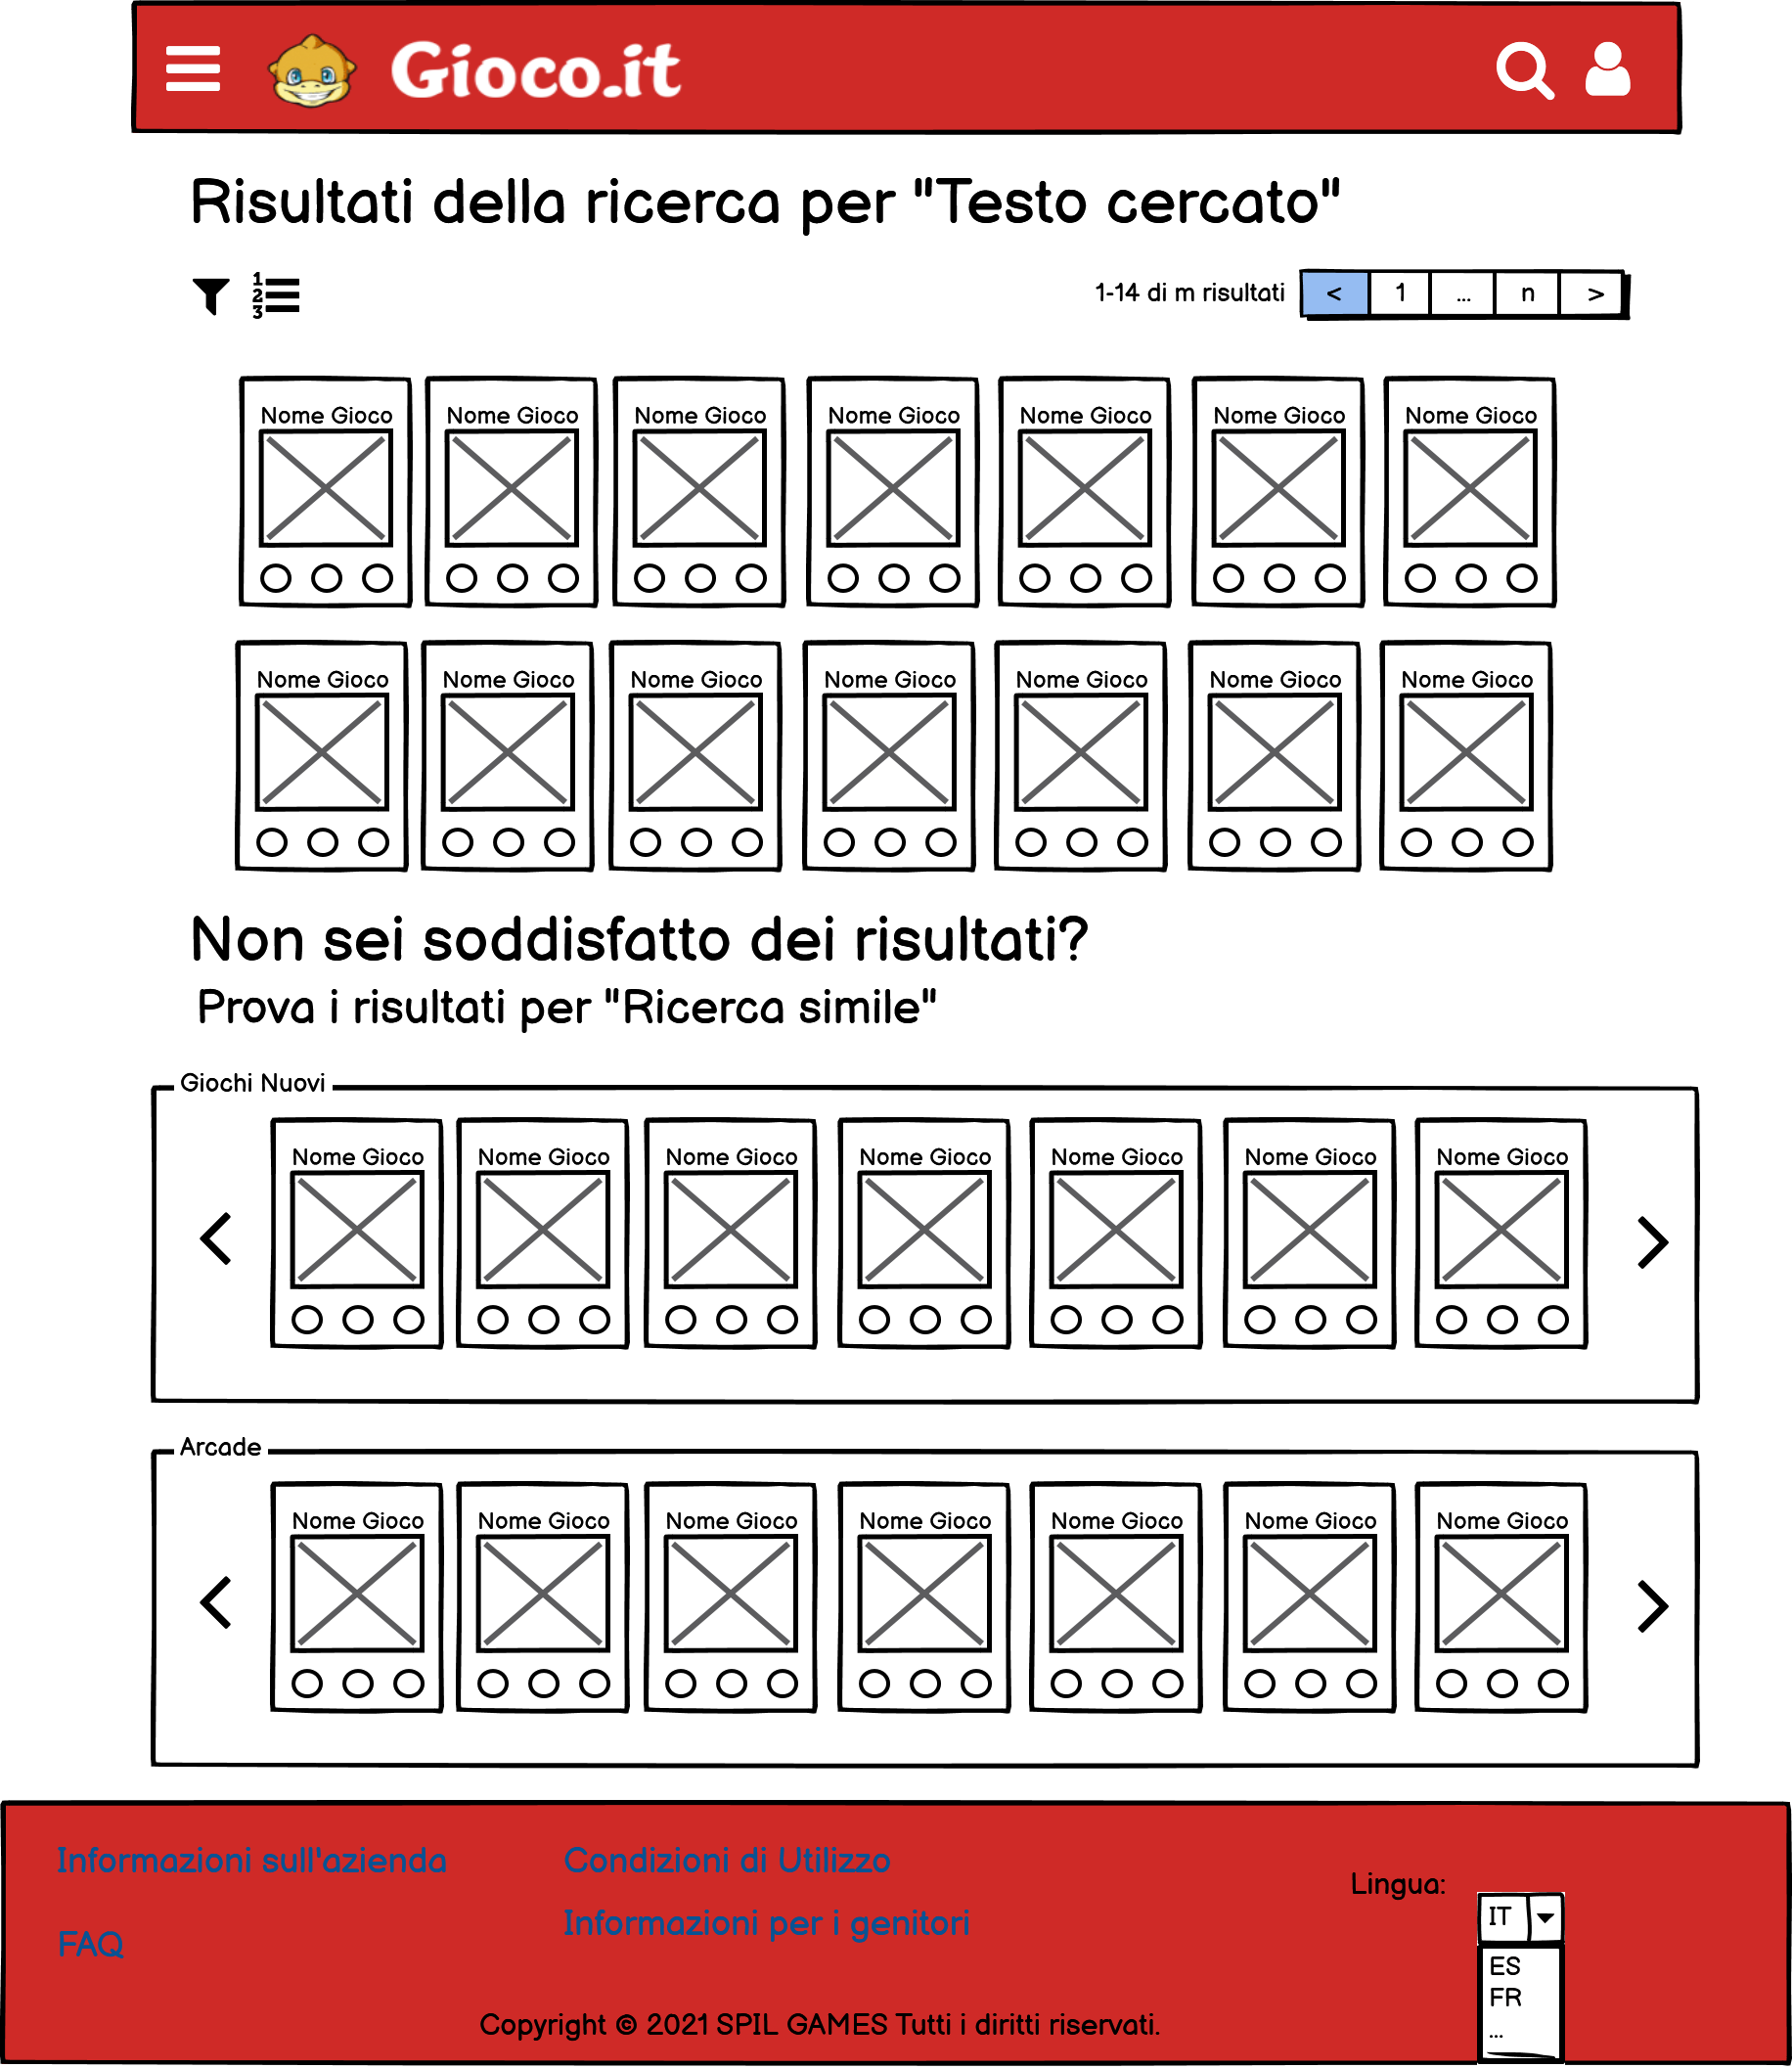
\includegraphics[width=8cm]{WSearchResult.png}
        \end{minipage}
    \end{figure}
    Qualora la ricerca non desse risultati verrá mostrata la pagina di sinistra dove in basso troviamo altri titoli che possono piacere.
    Se la ricerca invece ha dato un numero di risultati, questo lo troveremo in alto a destra insieme al numero di pagina. Troviamo inoltre 2 pulsanti per il filtro e l'ordinamento(nella vecchia versione del sito non erano presenti) e in basso troviamo due liste di giochi 'Suggeriti' qualora l'utente non sia soddisfatto dei risultati della ricerca.

    \subsection{Menu}
    Da modificare   
    
    \subsection{Categoria}
    Da aggiungere

    \subsection{Gioco}
    \begin{figure}[H]
        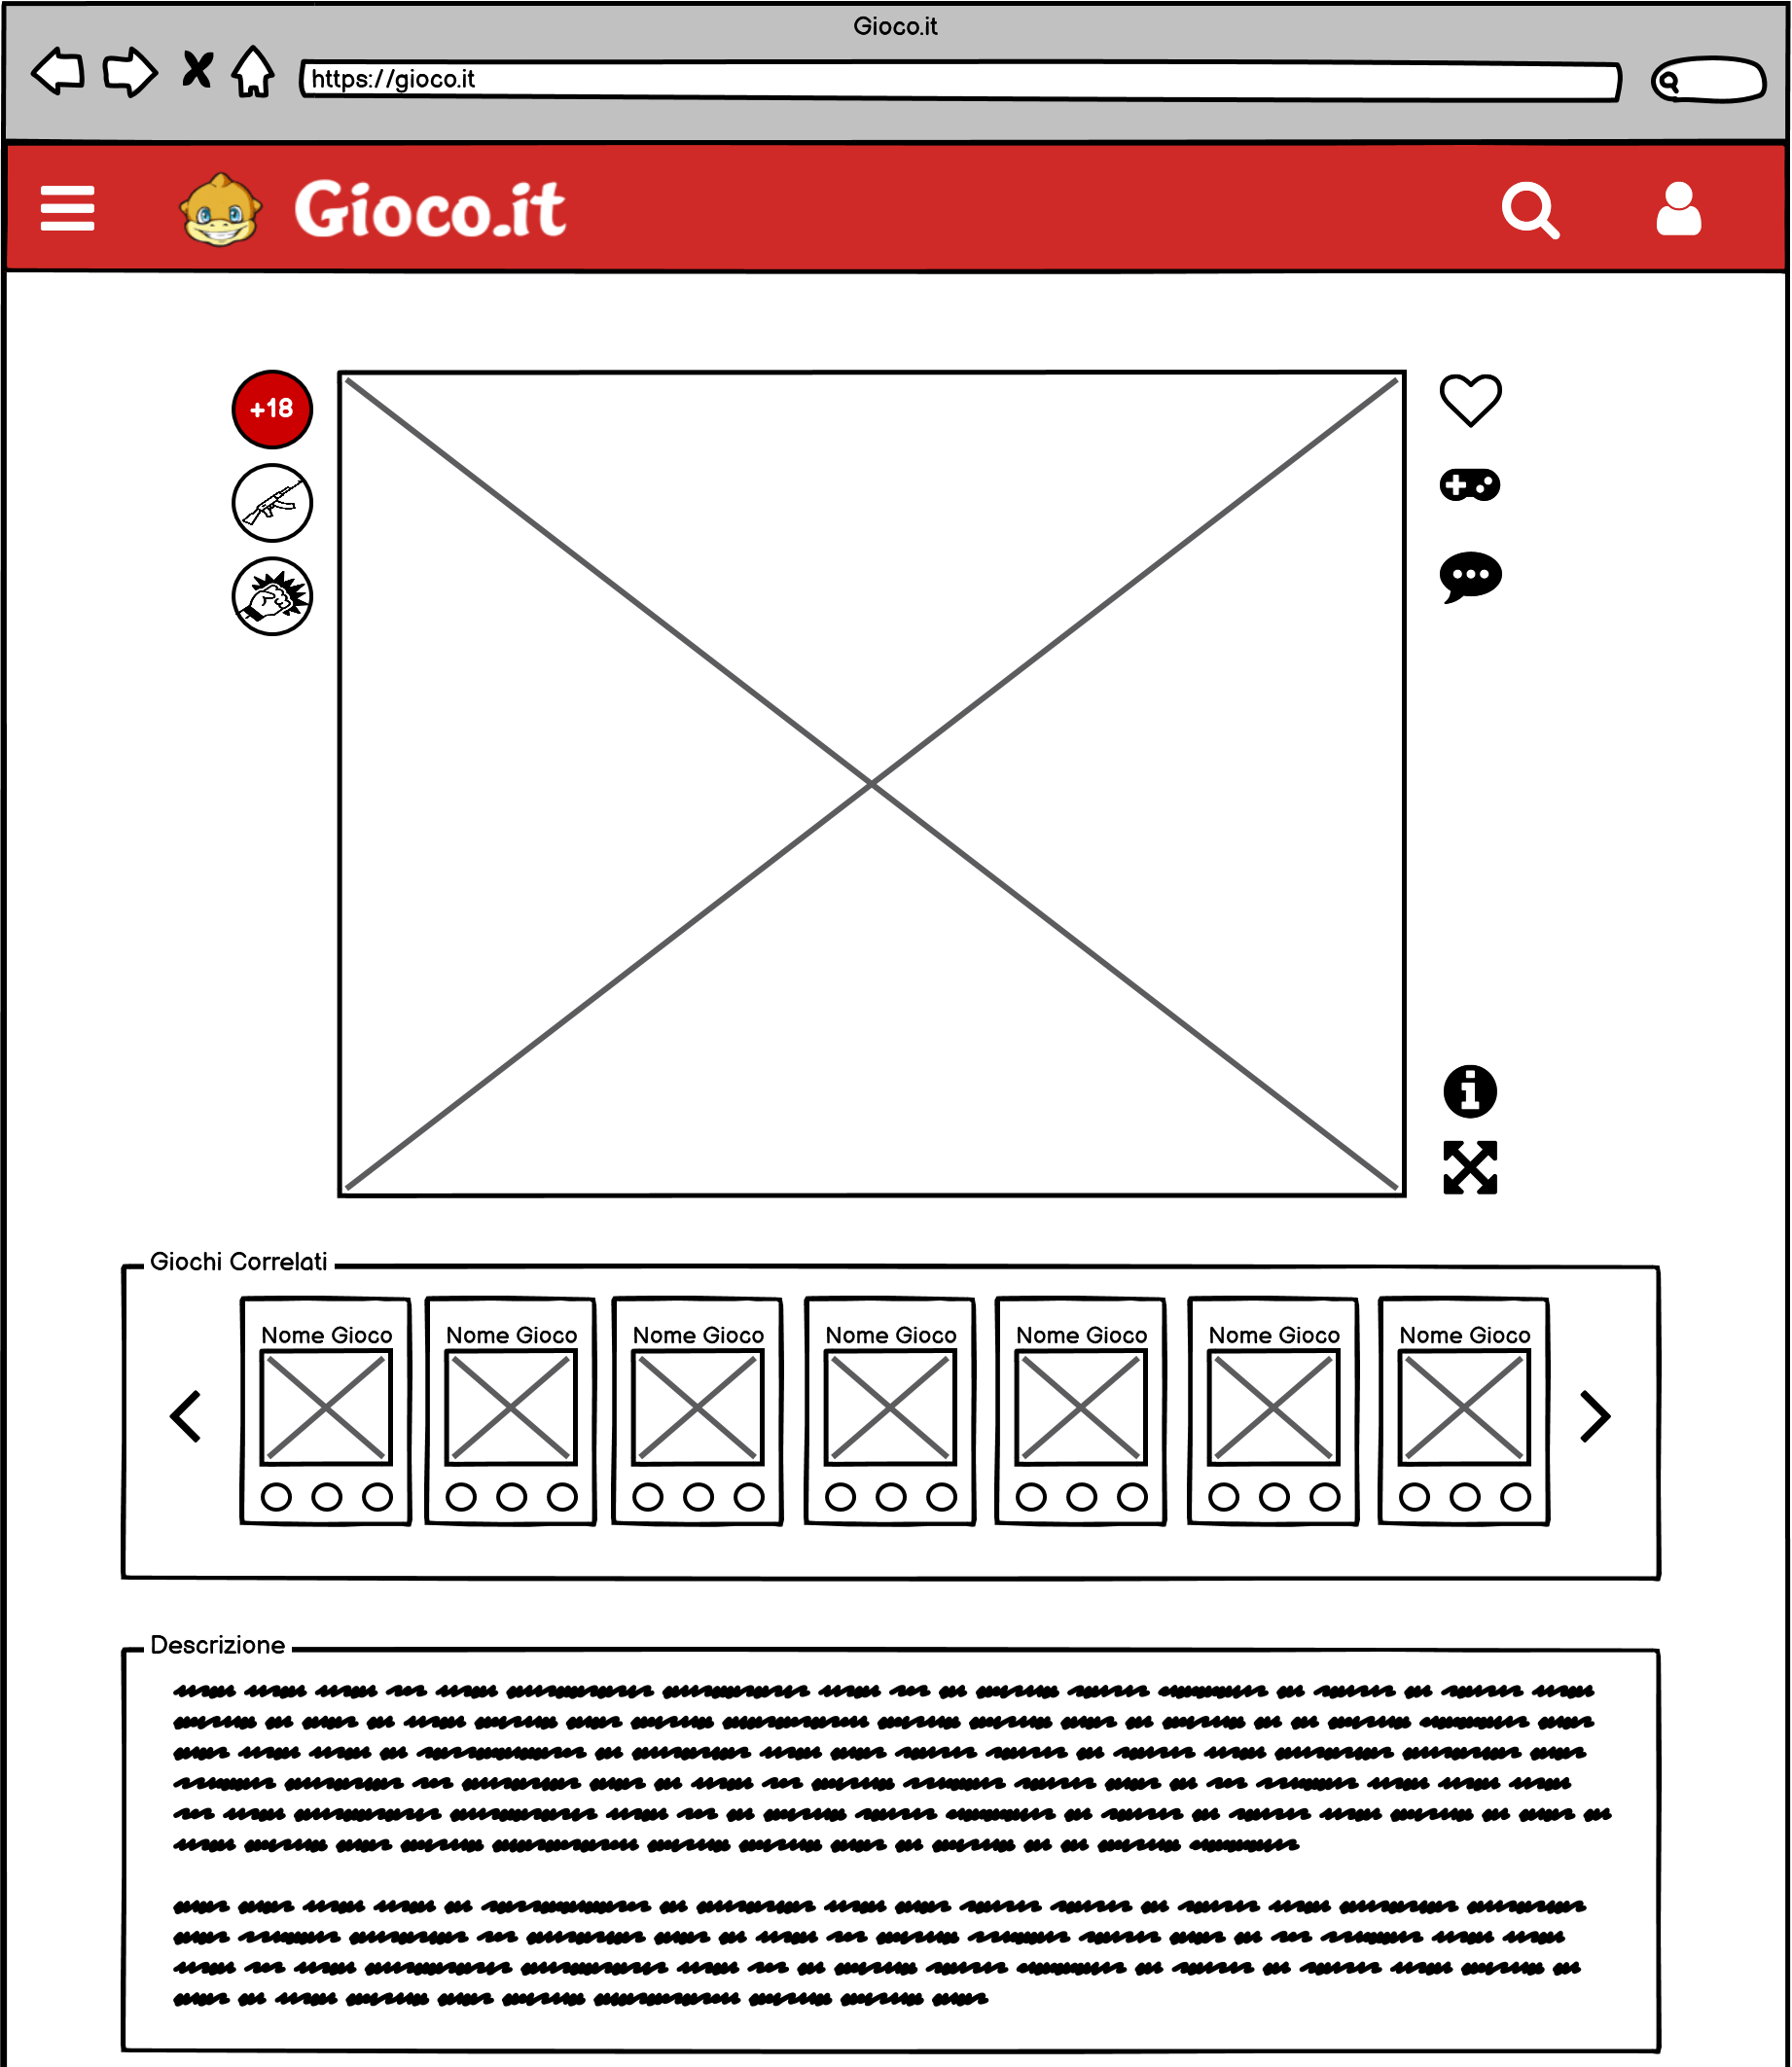
\includegraphics[width=10cm]{WGioco_1.png}
        \centering
    \end{figure}
    In primo piano abbiamo il riquadro di gioco, che è possibile ingrandire tramite il pulsante laterale di full screen in basso a destra. Abbiamo spostato la barra laterale dei pulsanti a sinistra e cambiato il pulsante dei preferiti (usando un cuore) rendendolo coerente con quello dei giochi preferiti all'interno della sezione profilo. Gli altri pulsanti rimandano a delle sotto sezioni della schermata di gioco cioè, seguendo l'ordine, quella della descrizione del gioco, dei commenti e del video tutorial del gioco.\\
    \\
    Rispetto al vecchio design, abbiamo tenuto soltanto la sezione orizzontale dei giochi correlati, eliminando anche quella laterale verticale, fatto per diminuire il carico cognitivo dell'utente.\\

    \begin{figure}[H]
        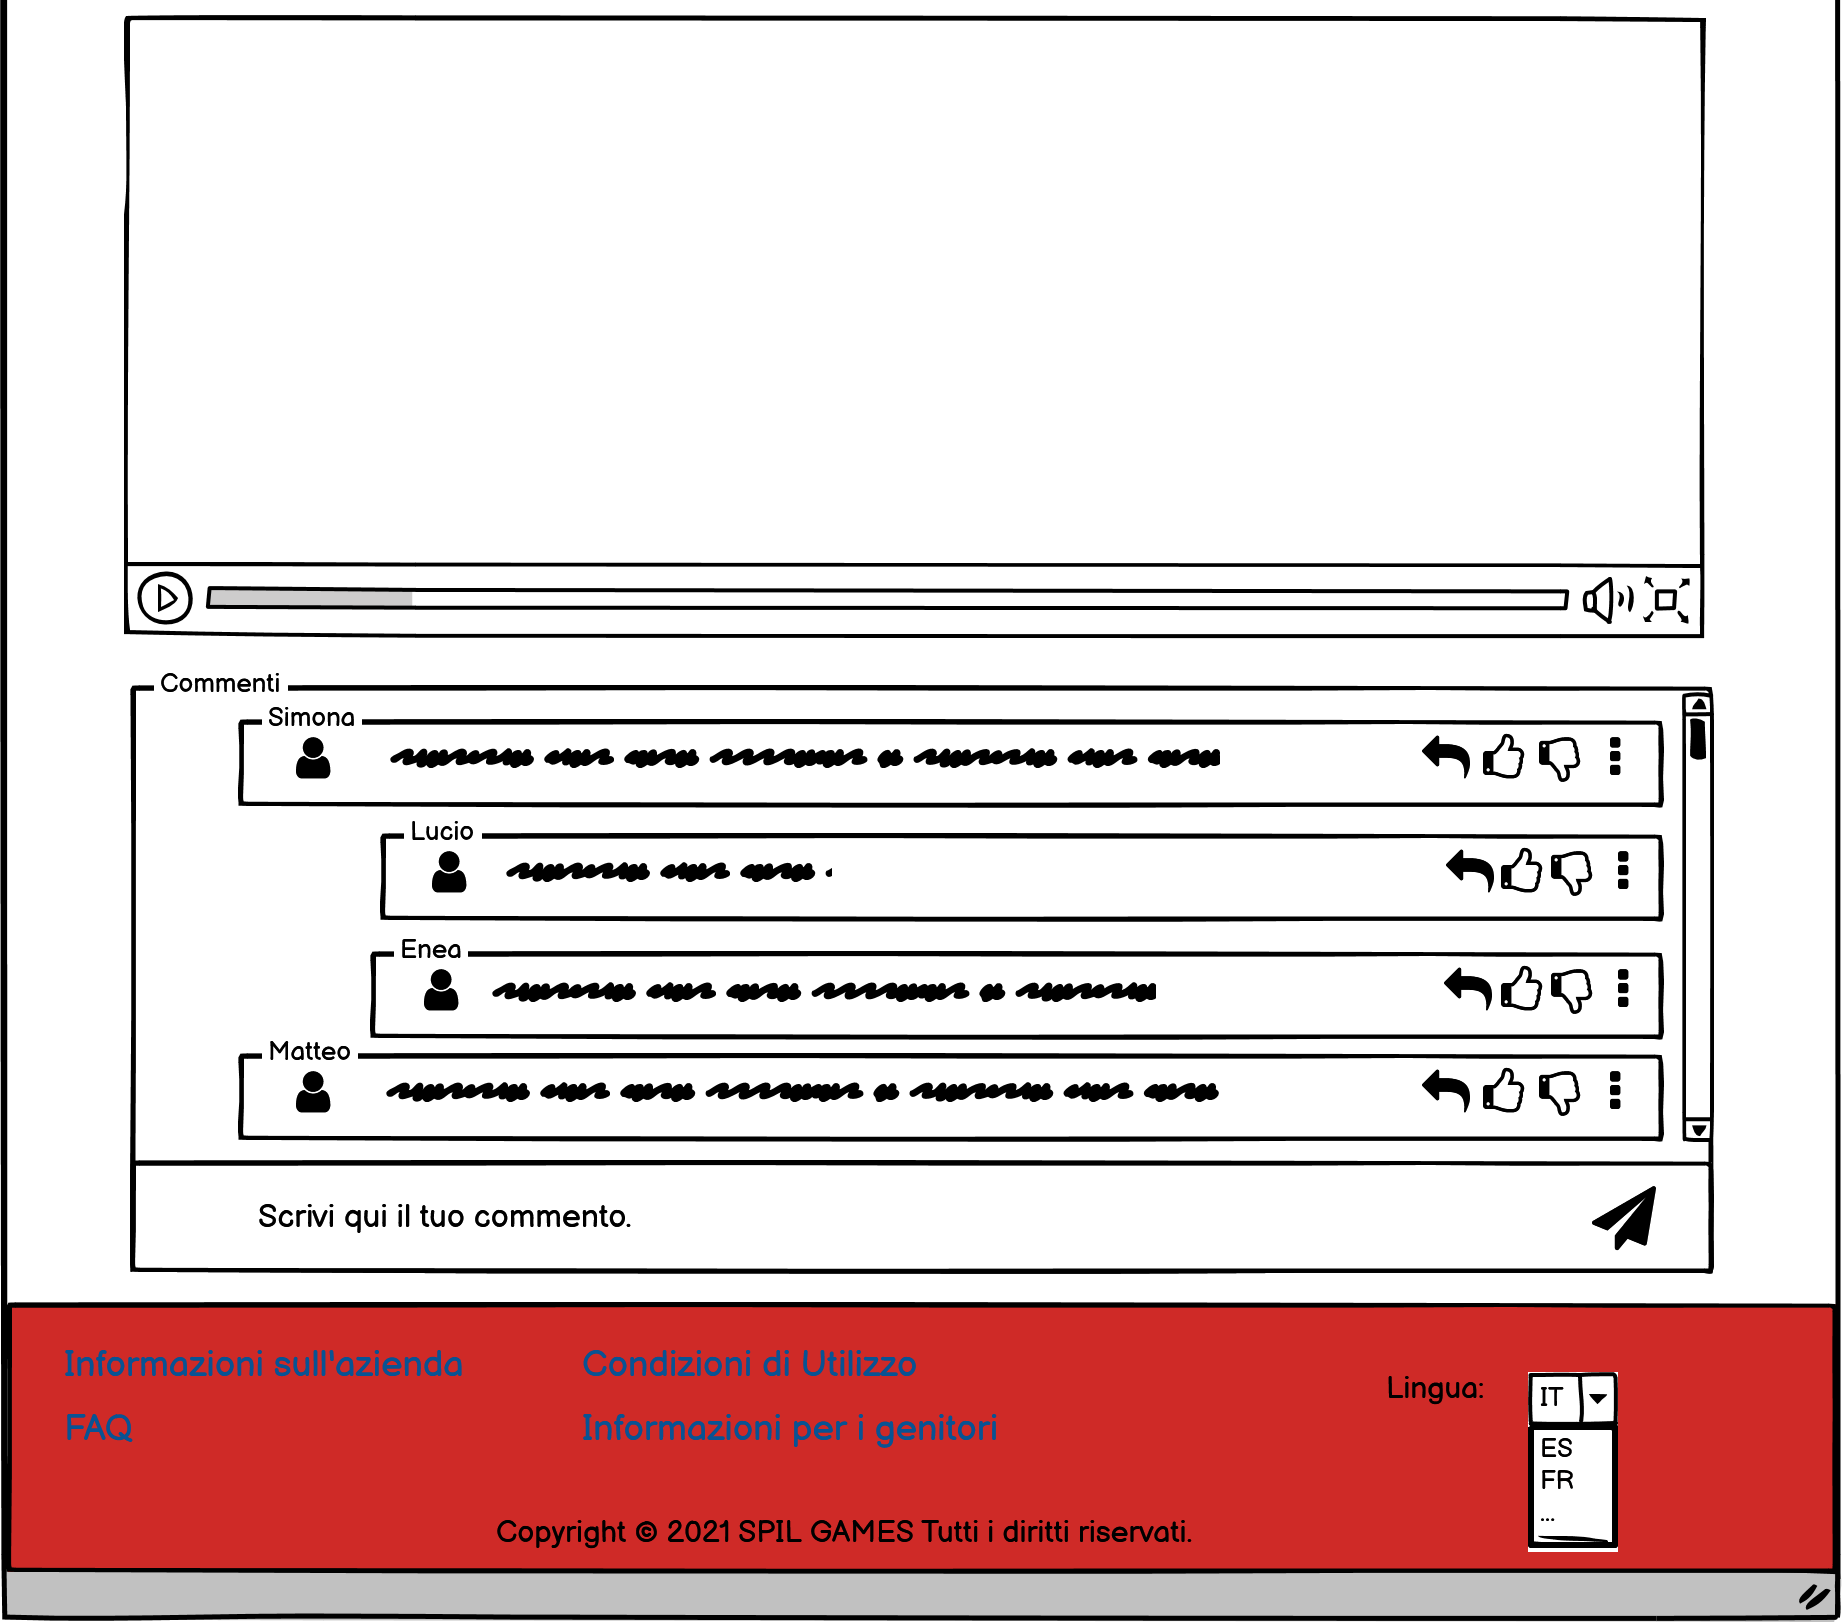
\includegraphics[width=10cm]{WGioco_2.png}
        \centering
    \end{figure}

    La sotto sezione della descrizone del gioco e quella del video tutorial sono rimaste invariate, nella prima verrà descritto lo scopo del gioco e i comandi da utilizzare per giocarci. Anche la parte dei commenti rimane pressoché invariata, se non per qualche modifica dei pulsanti per renderla più intuitiva e, ovviamente, per utilizzarla bisogna eseguire l'accesso al profilo. Con essa è possibile scrivere commenti e rispondere ad essi )(creando delle conversazioni), mettere like o dislike a commenti di altre persone, condividerli o segnalarli (tramite il pulsante dei tre puntini).


    \subsection{Profilo}
    La sezione profilo è stata totalmente ridisegnata, in questo modo:
    \begin{figure}[H]
        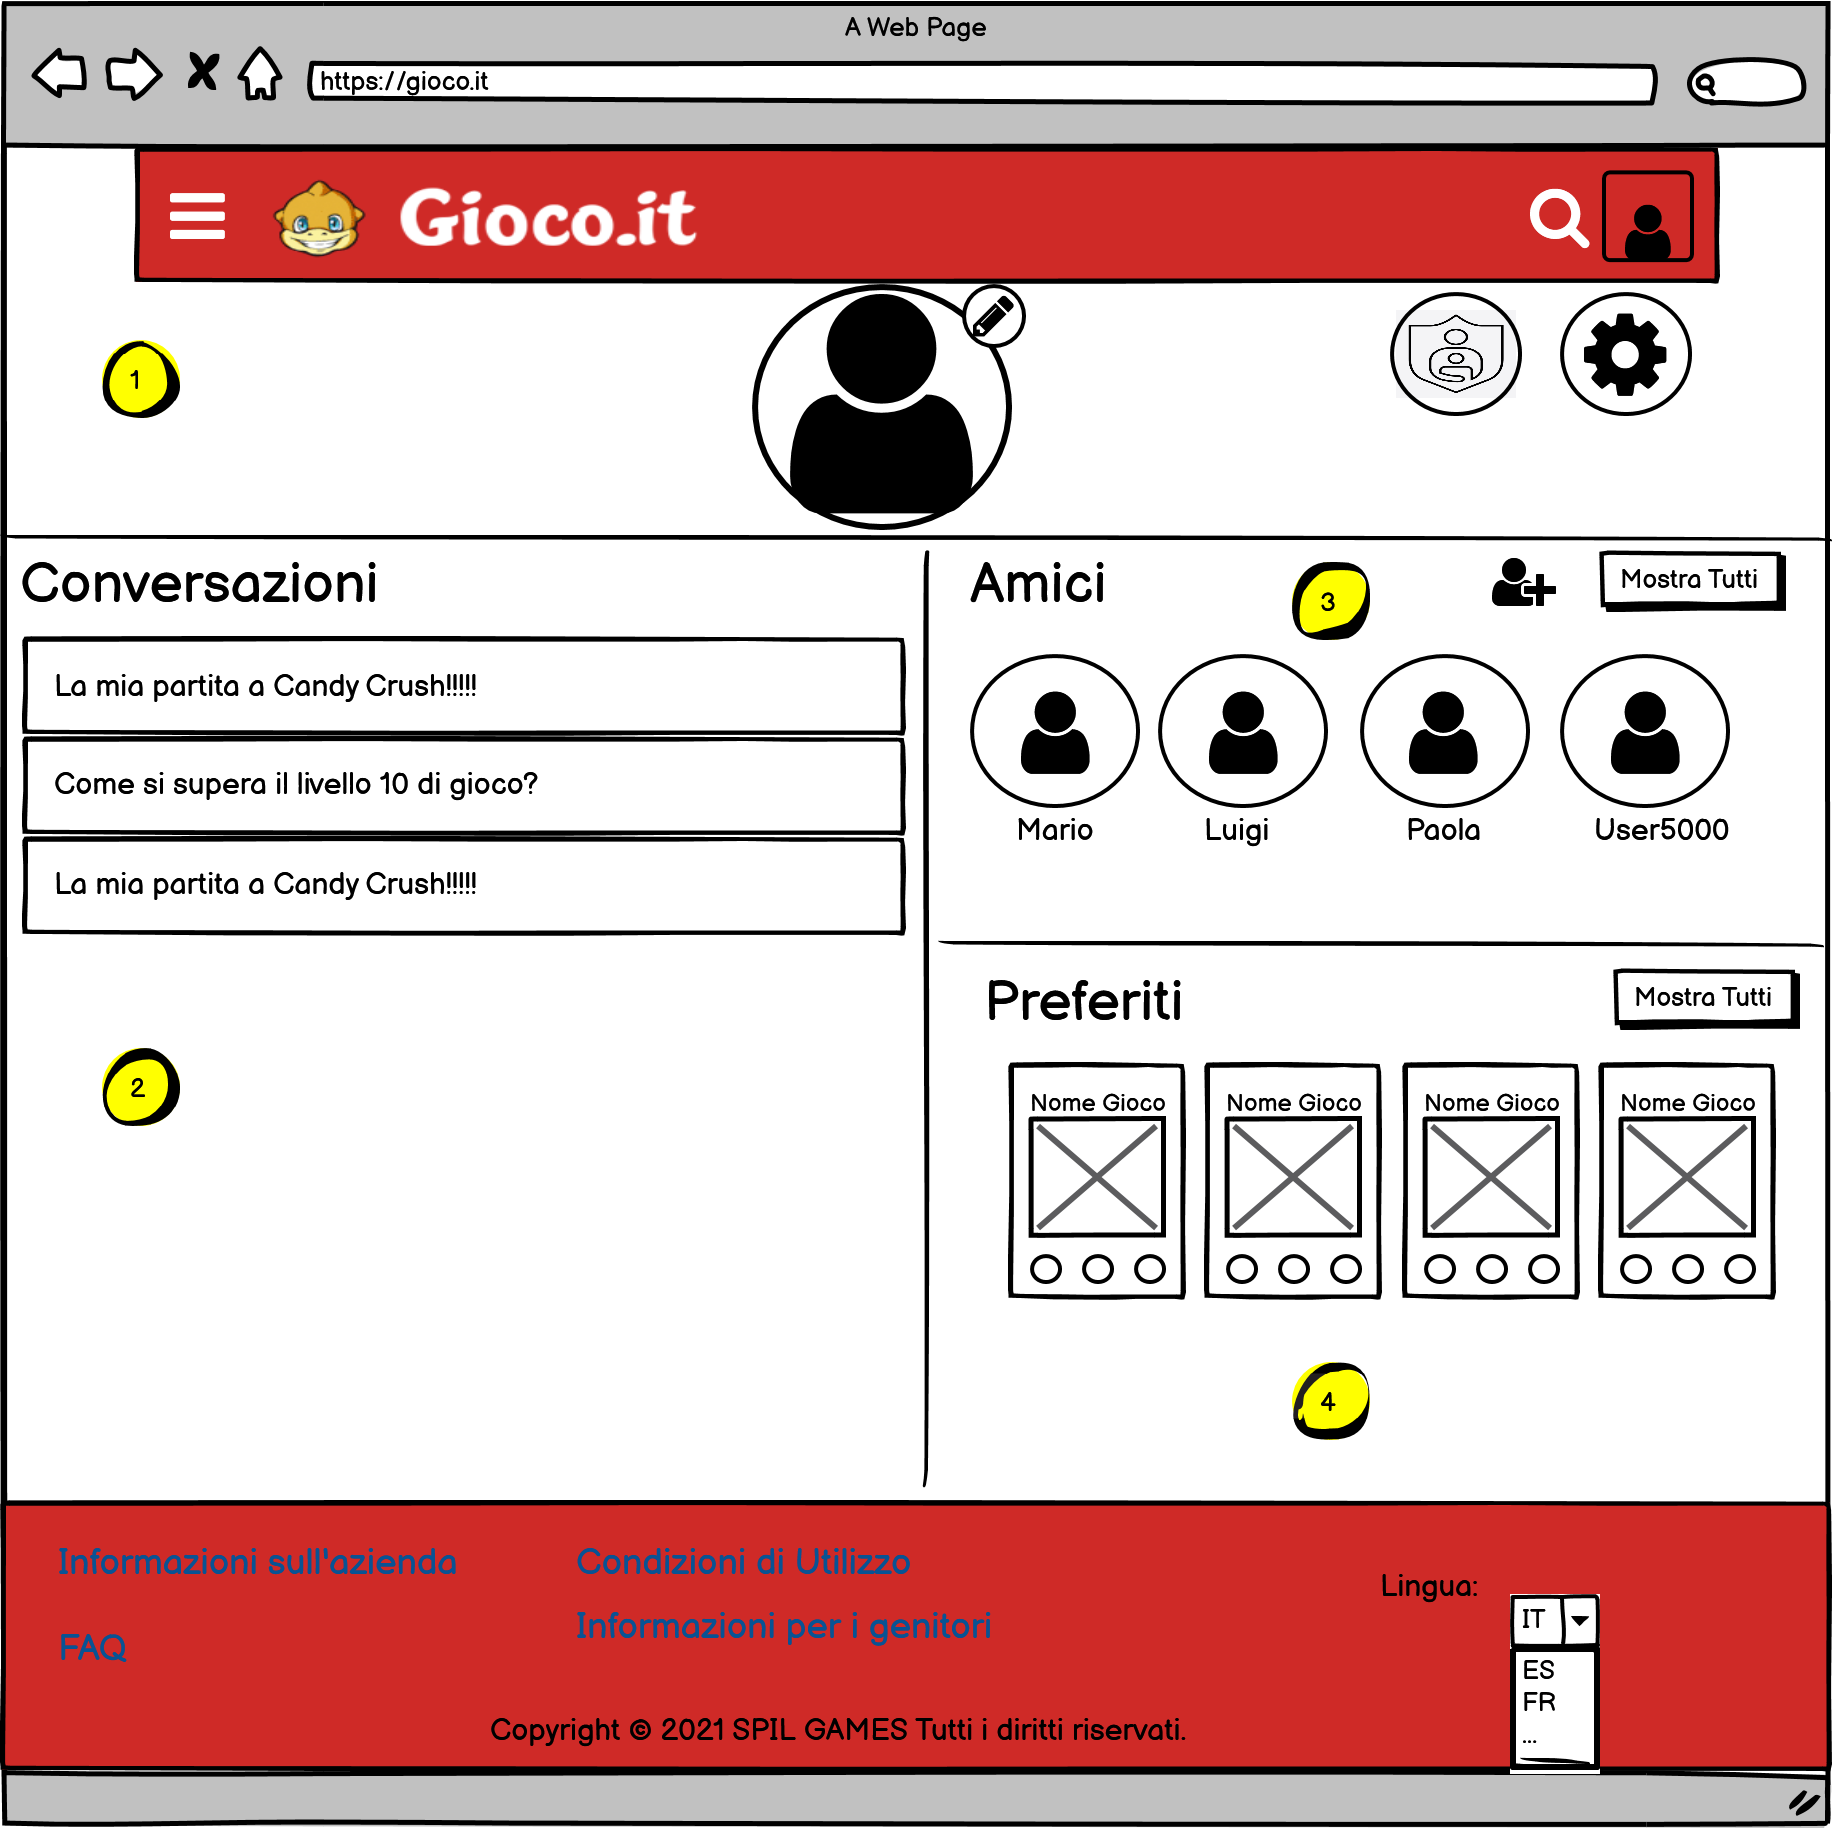
\includegraphics[width=10cm]{WProfile.png}
        \centering
    \end{figure}
    
    Possiamo vederla come quattro sotto sezioni:
    \begin{enumerate}
        \item Immagine del profilo con i pulsanti impostazioni e parental control
        \item Conversazioni attive
        \item Lista di amici con i pulsanti di aggiunta amico e mostra tutti
        \item Lista delle card dei giochi preferiti con il pulsante "mostra tutti".
    \end{enumerate}

    \subsubsection{Sotto sezione 1}
    Qui è contenuta l'immagine del profilo, modificabile, infatti al click sulla matita verremo spostati nella seguente schermata di modifica dell'immagine:
    \begin{figure}[H]
        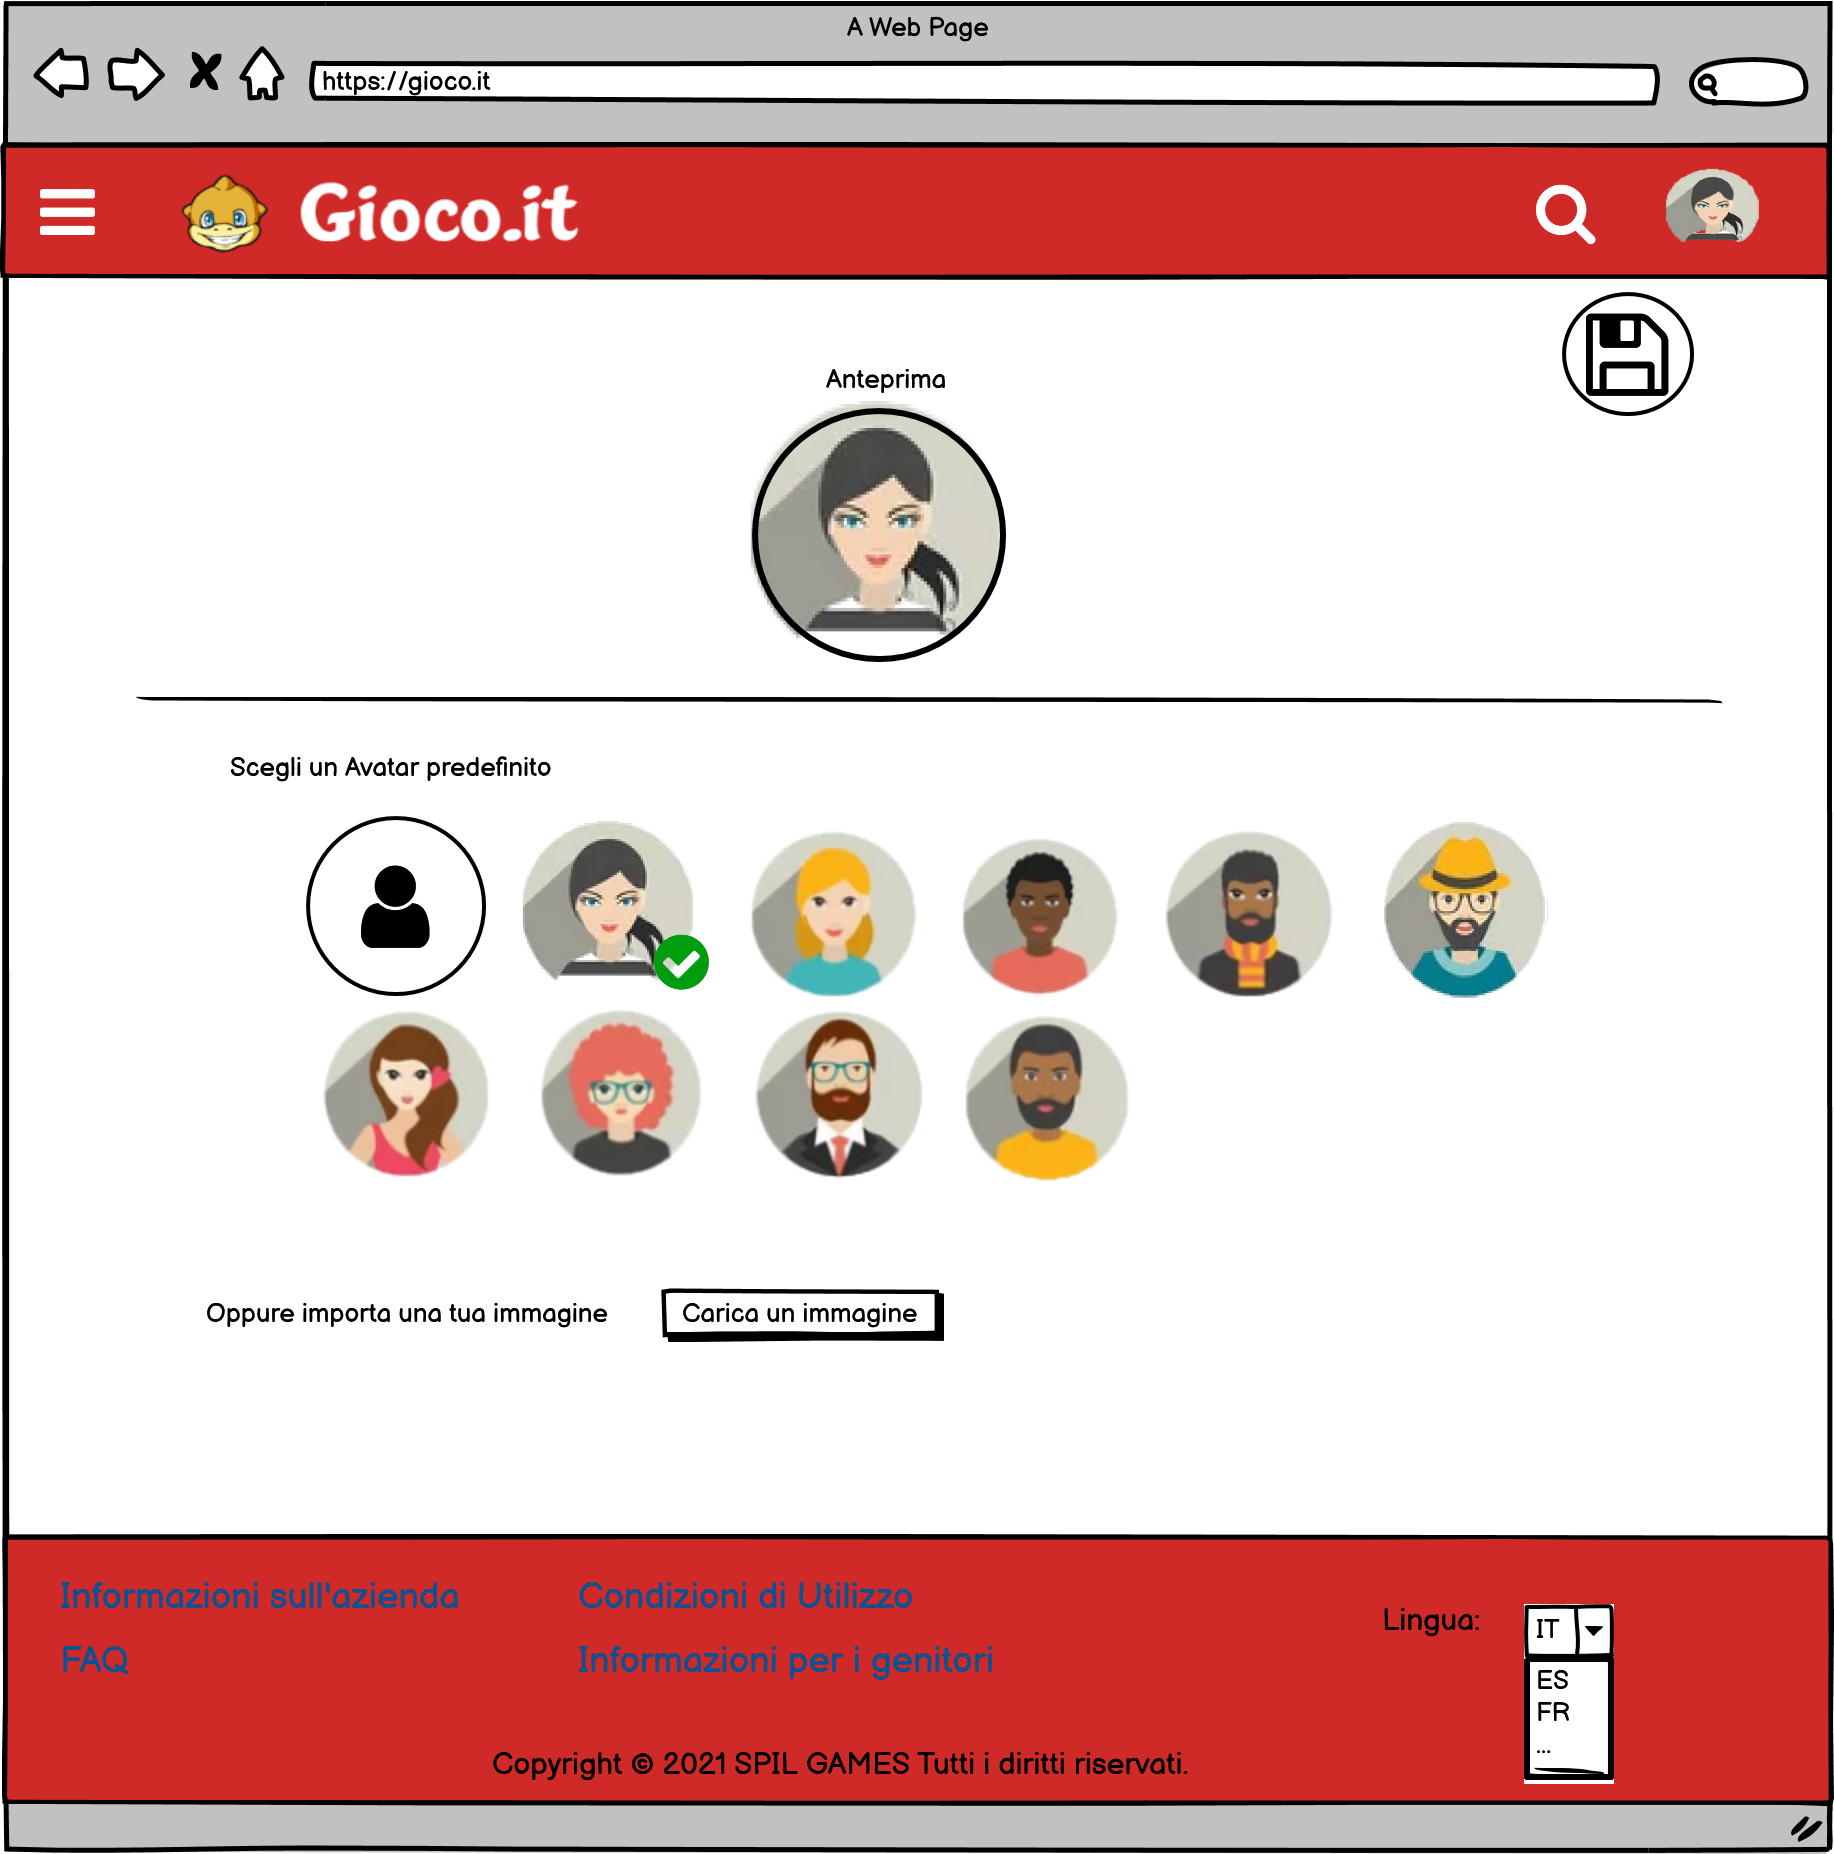
\includegraphics[width=10cm]{WImageProfile.png}
        \centering
    \end{figure}
    Dove sarà possibile selezionare un avatar di quelli già presenti oppure caricare un'immagine localmente e salvare.\\
    \\
    Inoltre, in questa sotto sezione, ci sono anche i due pulsanti "impostazioni" e "parental control", dove il primo ci condurrà alla seguente schermata:
    \begin{figure}[H]
        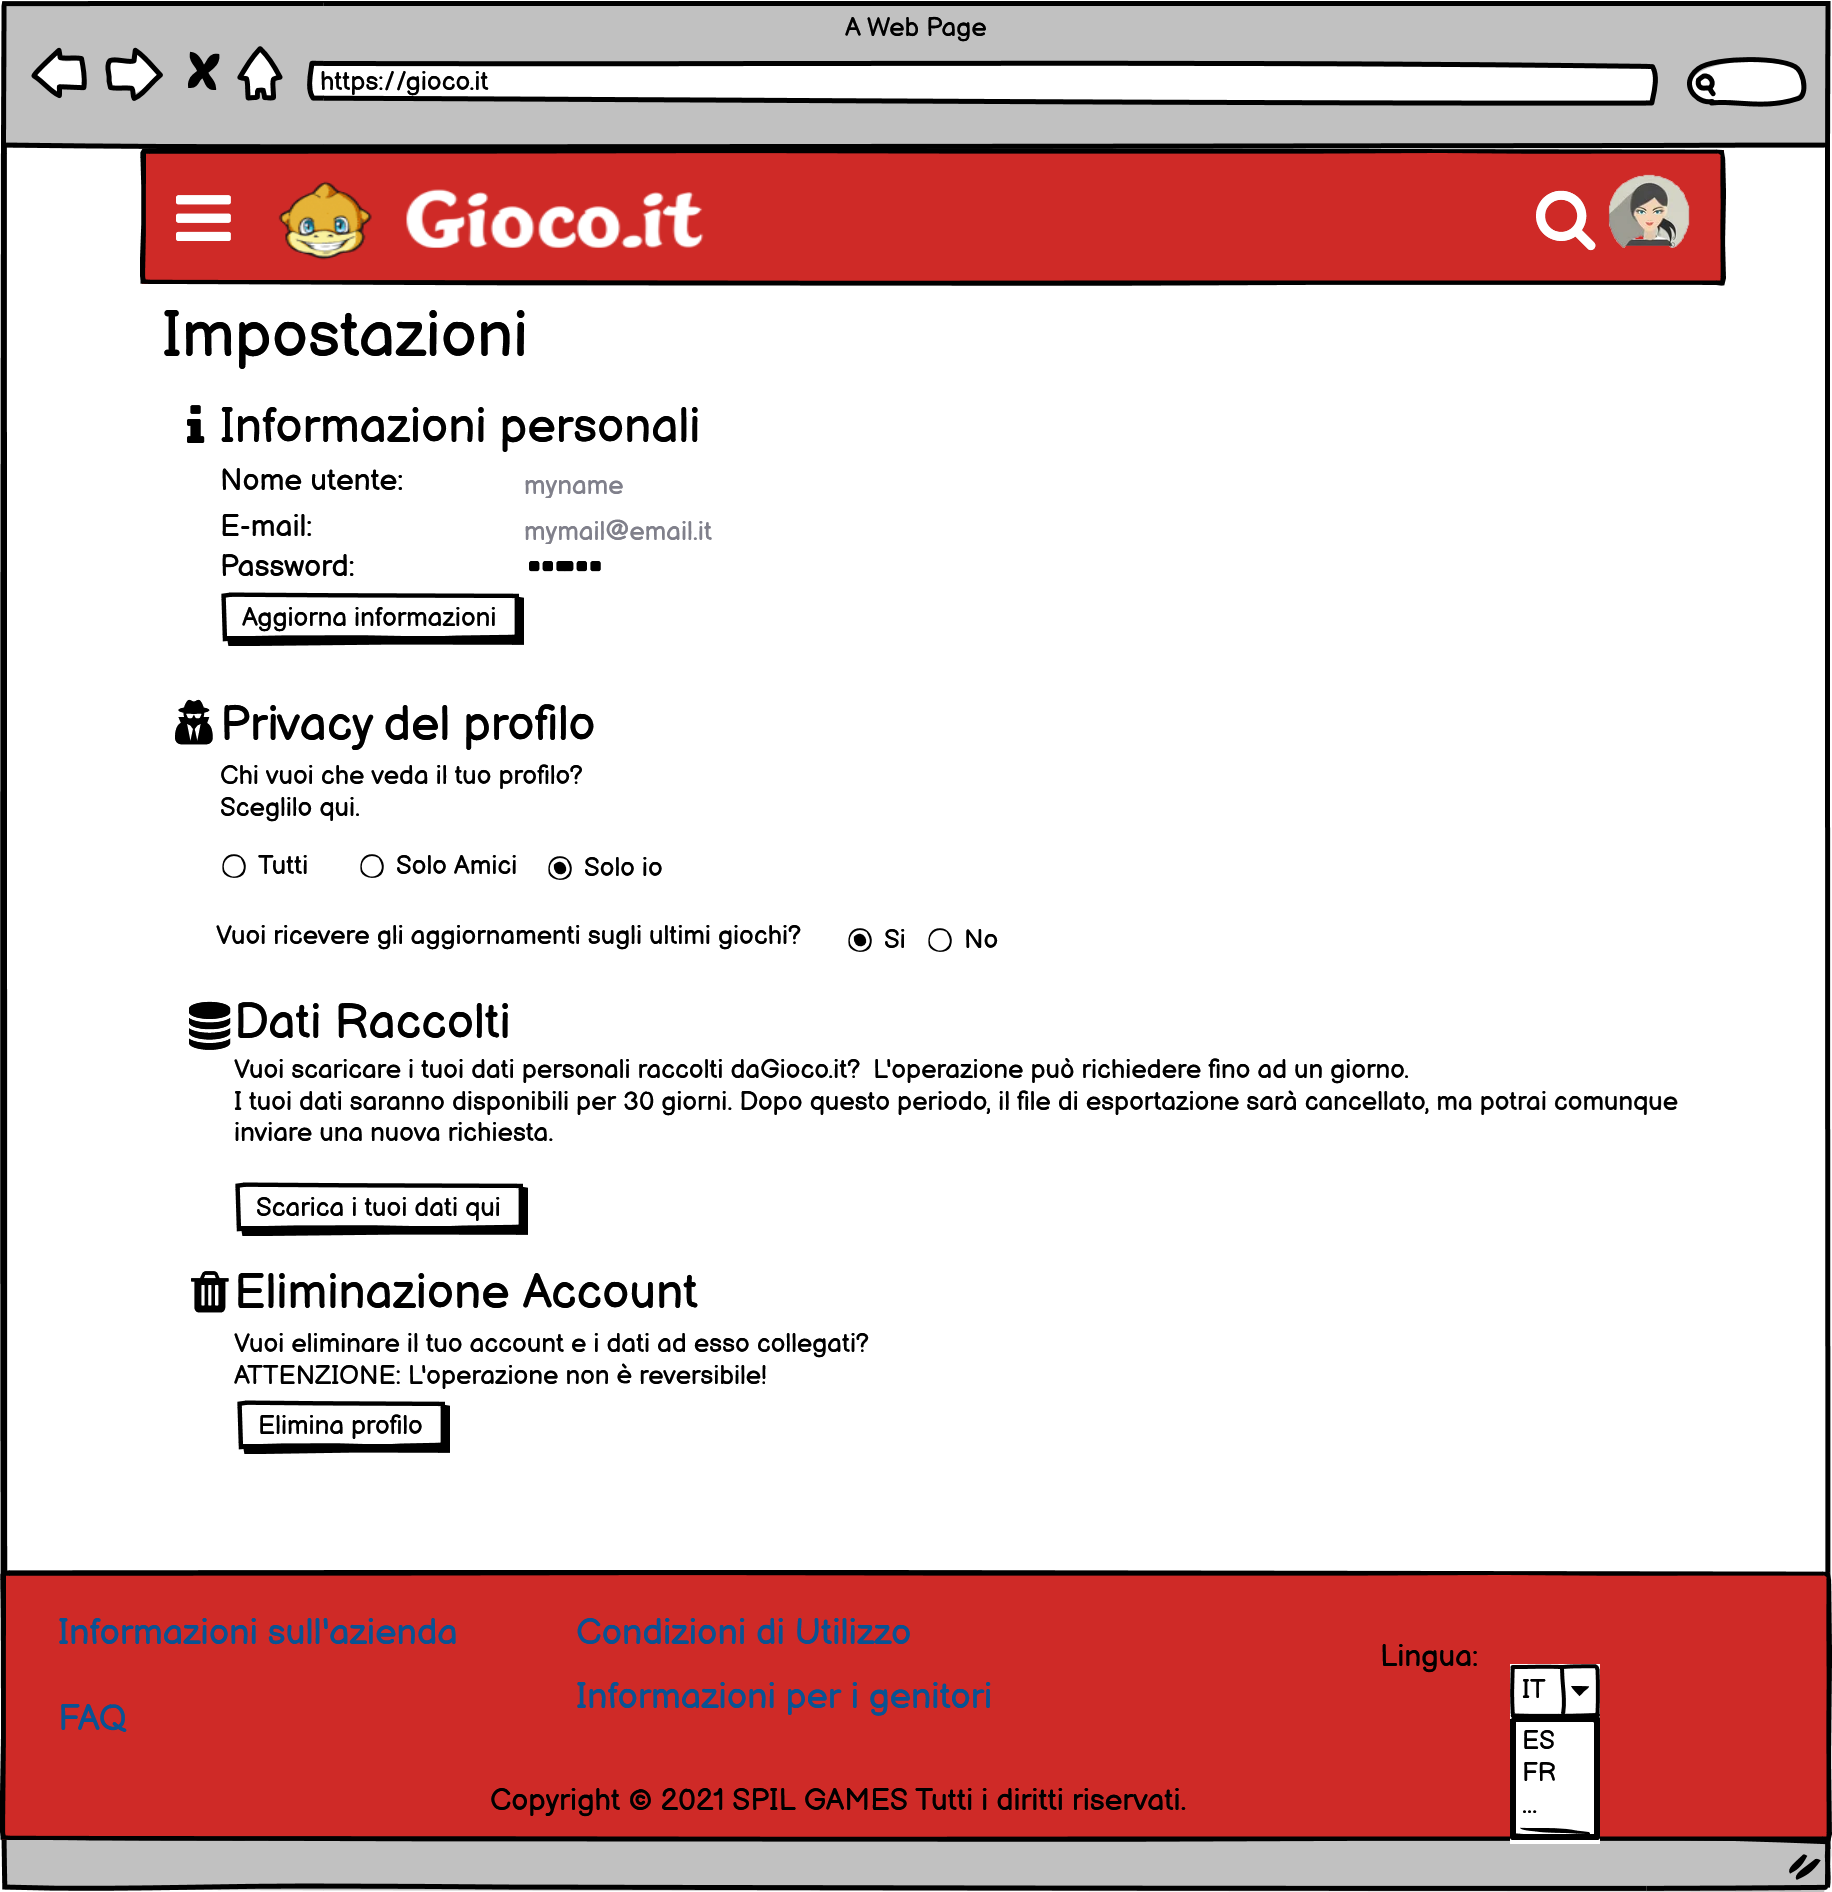
\includegraphics[width=10cm]{WImpostazioni.png}
        \centering
    \end{figure}
    Dove sarà possibile aggiornare i propri dati personali, come nome utente, e-mail e password (nella vecchia versione era possibile modificare solo la password), modificare le impostazioni di privacy (chi può visualizzare il profilo), scaricare i dati personali raccolti su Gioco.it ed eliminare l'account.\\
    \\
    Mentre il secondo pulsante (parental control) ci condurrà ad una nuova schermata di impostazioni per i supervisori che vedremo più avanti (sezione \ref{section: parental control}).


    \subsubsection{Sotto sezione 2}
    In questa sotto sezione abbiamo, in ordine cronologico, le ultime conversazioni attive a cui abbiamo partecipato.

    \subsubsection{Sotto sezione 3}
    In questa sotto sezione si possono vedere gli ultimi amici aggiunti e c'è la possibilità, con due pulsanti diversi, di aggiungerne altri o mostrarli tutti.
    Nel caso si volessero vedere tutti gli amici si vedrà modificarsi la sezione corrente con una tab bar a tre tab:
    
    \begin{figure}[H]
        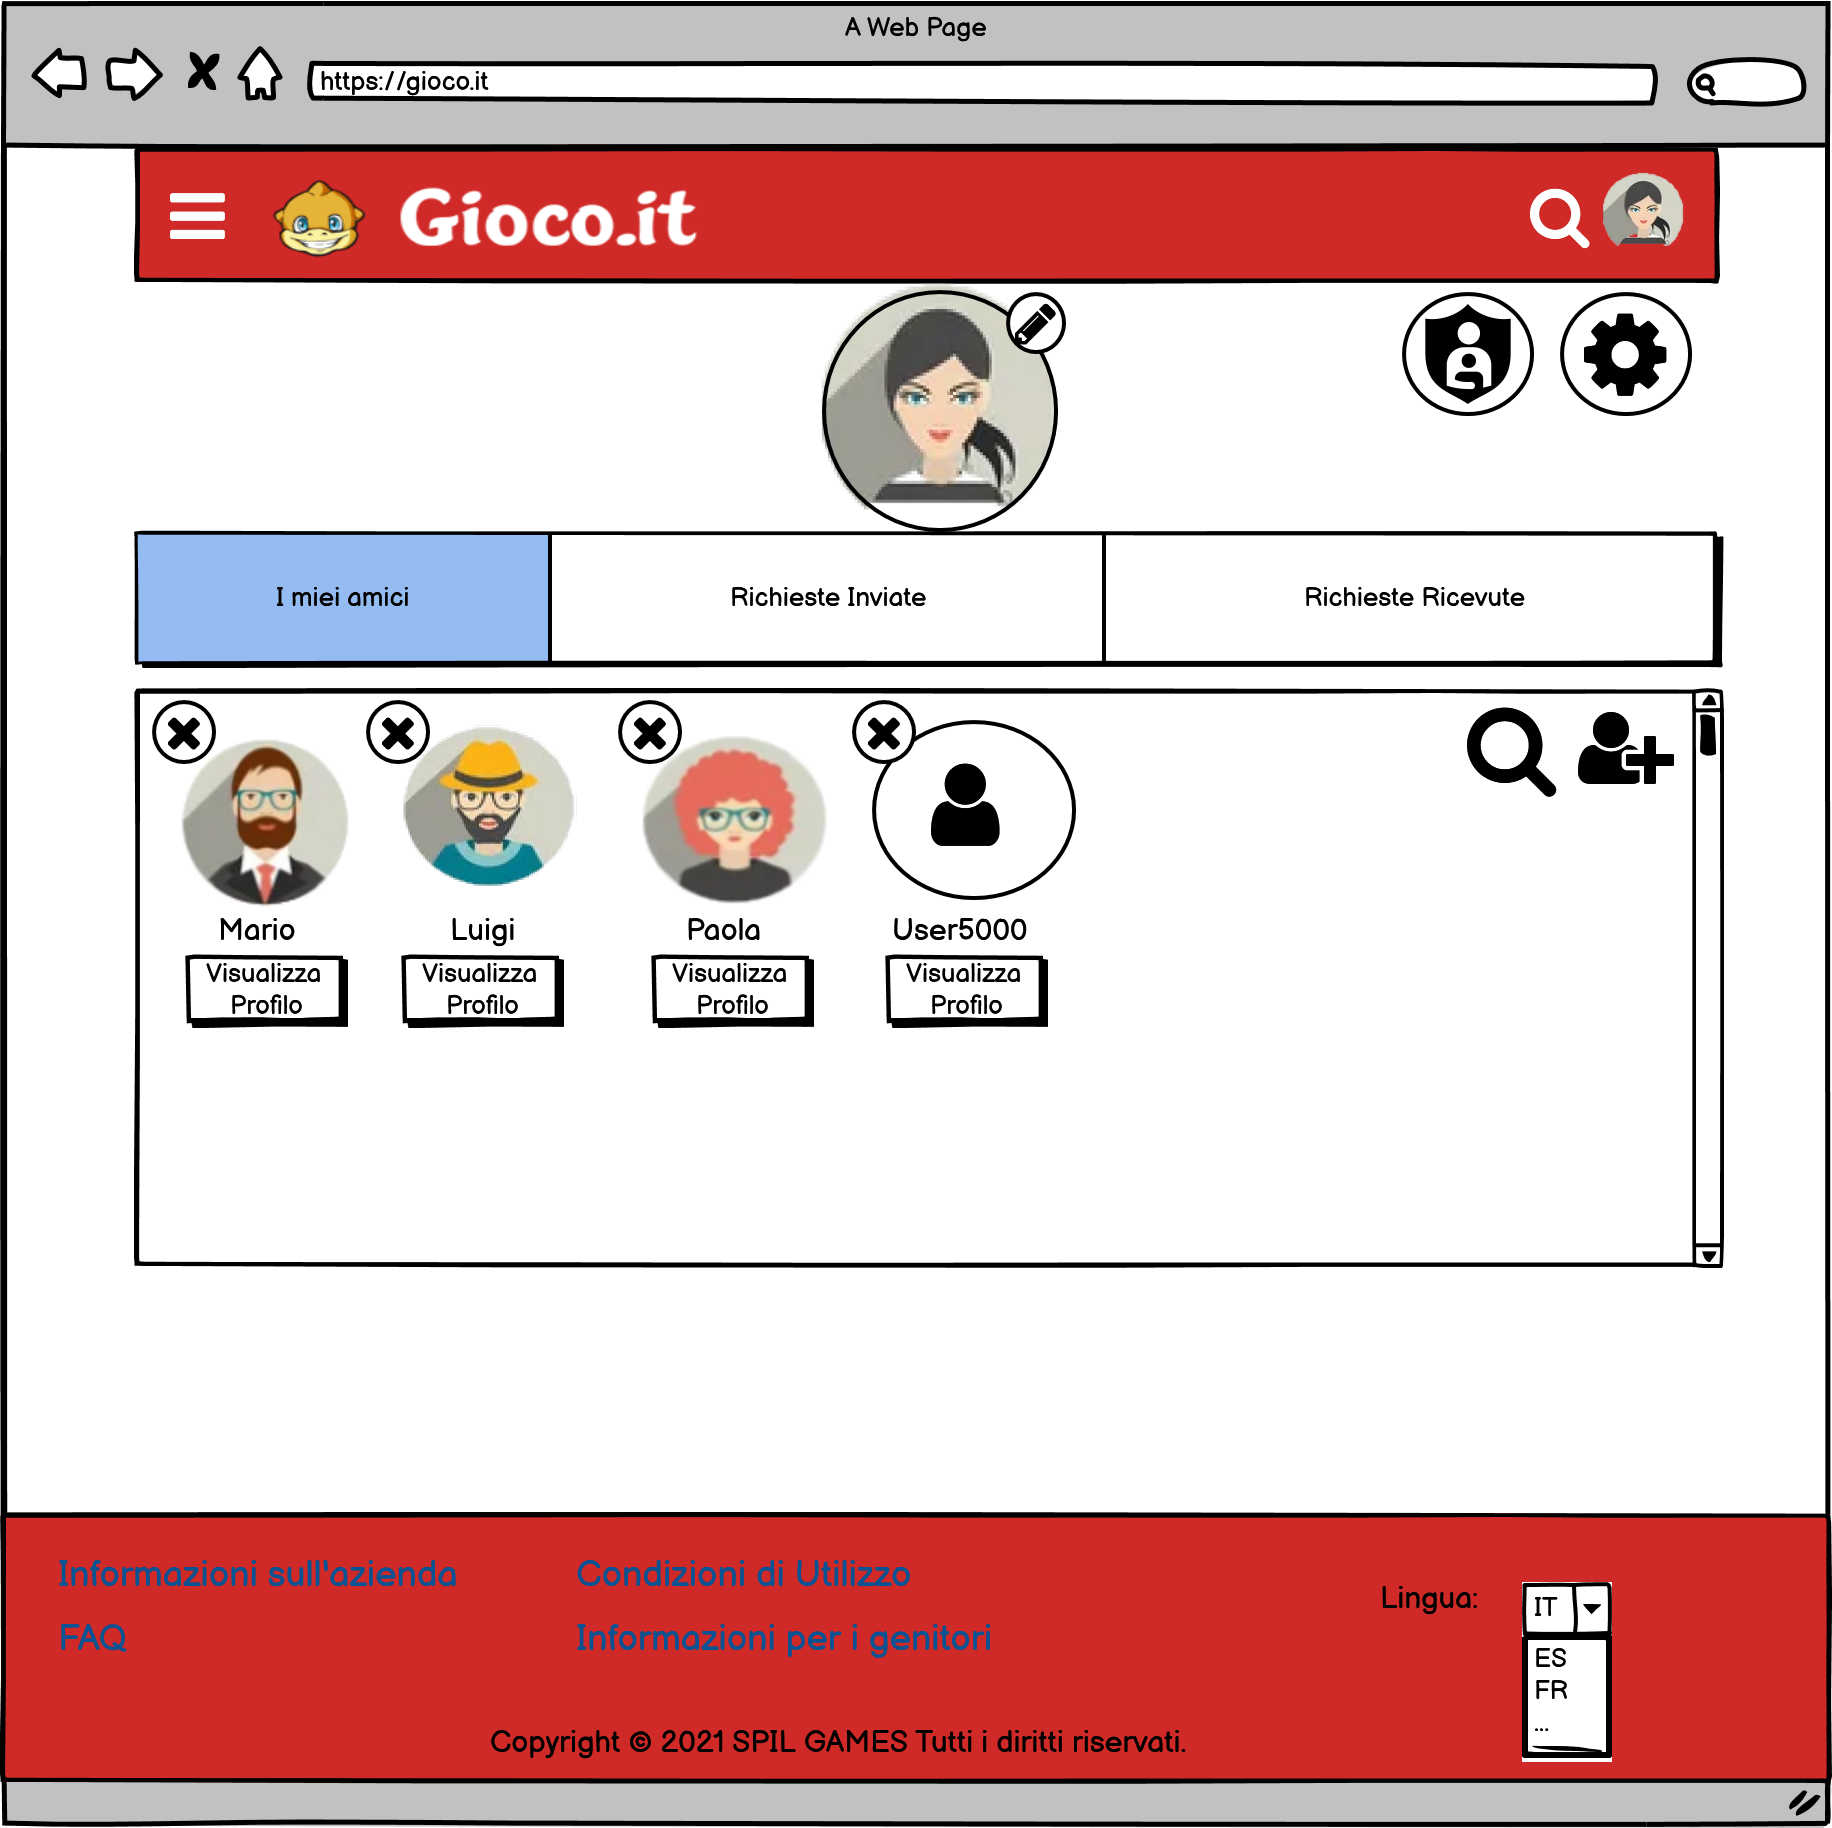
\includegraphics[width=10cm]{WAmici1.png}
        \centering
    \end{figure}

    Dove, in questa prima tab, vengono mostrati tutti gli amici con anche la possibilità di ricercarli per nome, cancellarli ed aggiungerne altri.

    \begin{figure}[H]
        \hspace{-1.5cm}
        \begin{minipage}[b]{8cm}
            \centering
            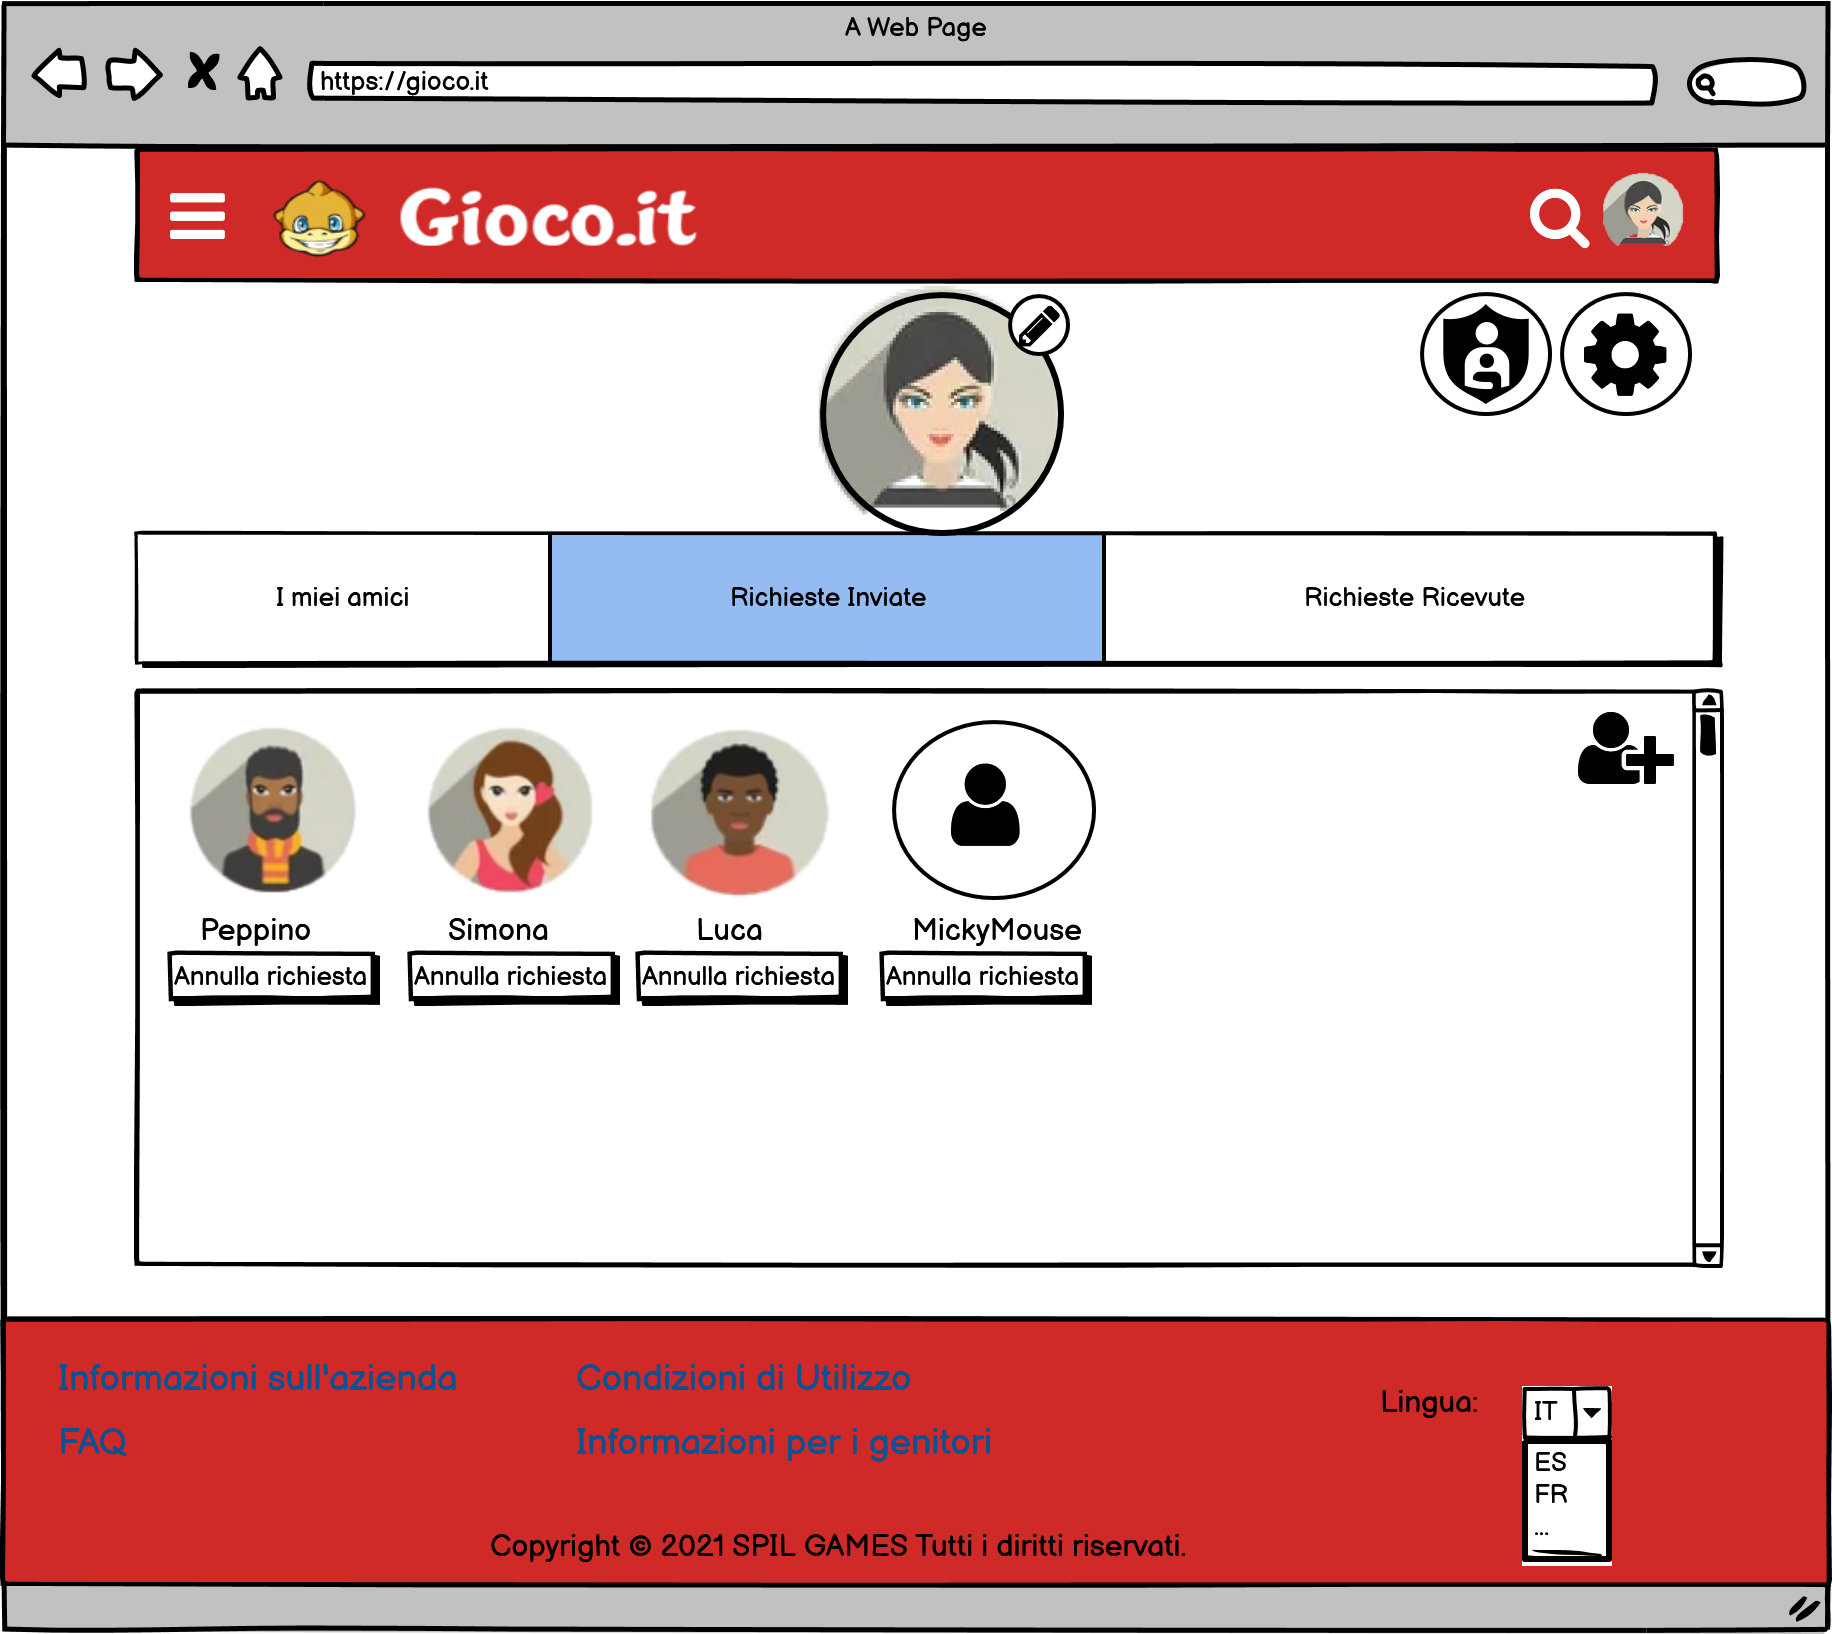
\includegraphics[width=8cm]{WAmici2.png}
            \end{minipage}
            \ \hspace{2mm} \hspace{3mm} \
            \begin{minipage}[b]{8cm}
            \centering
            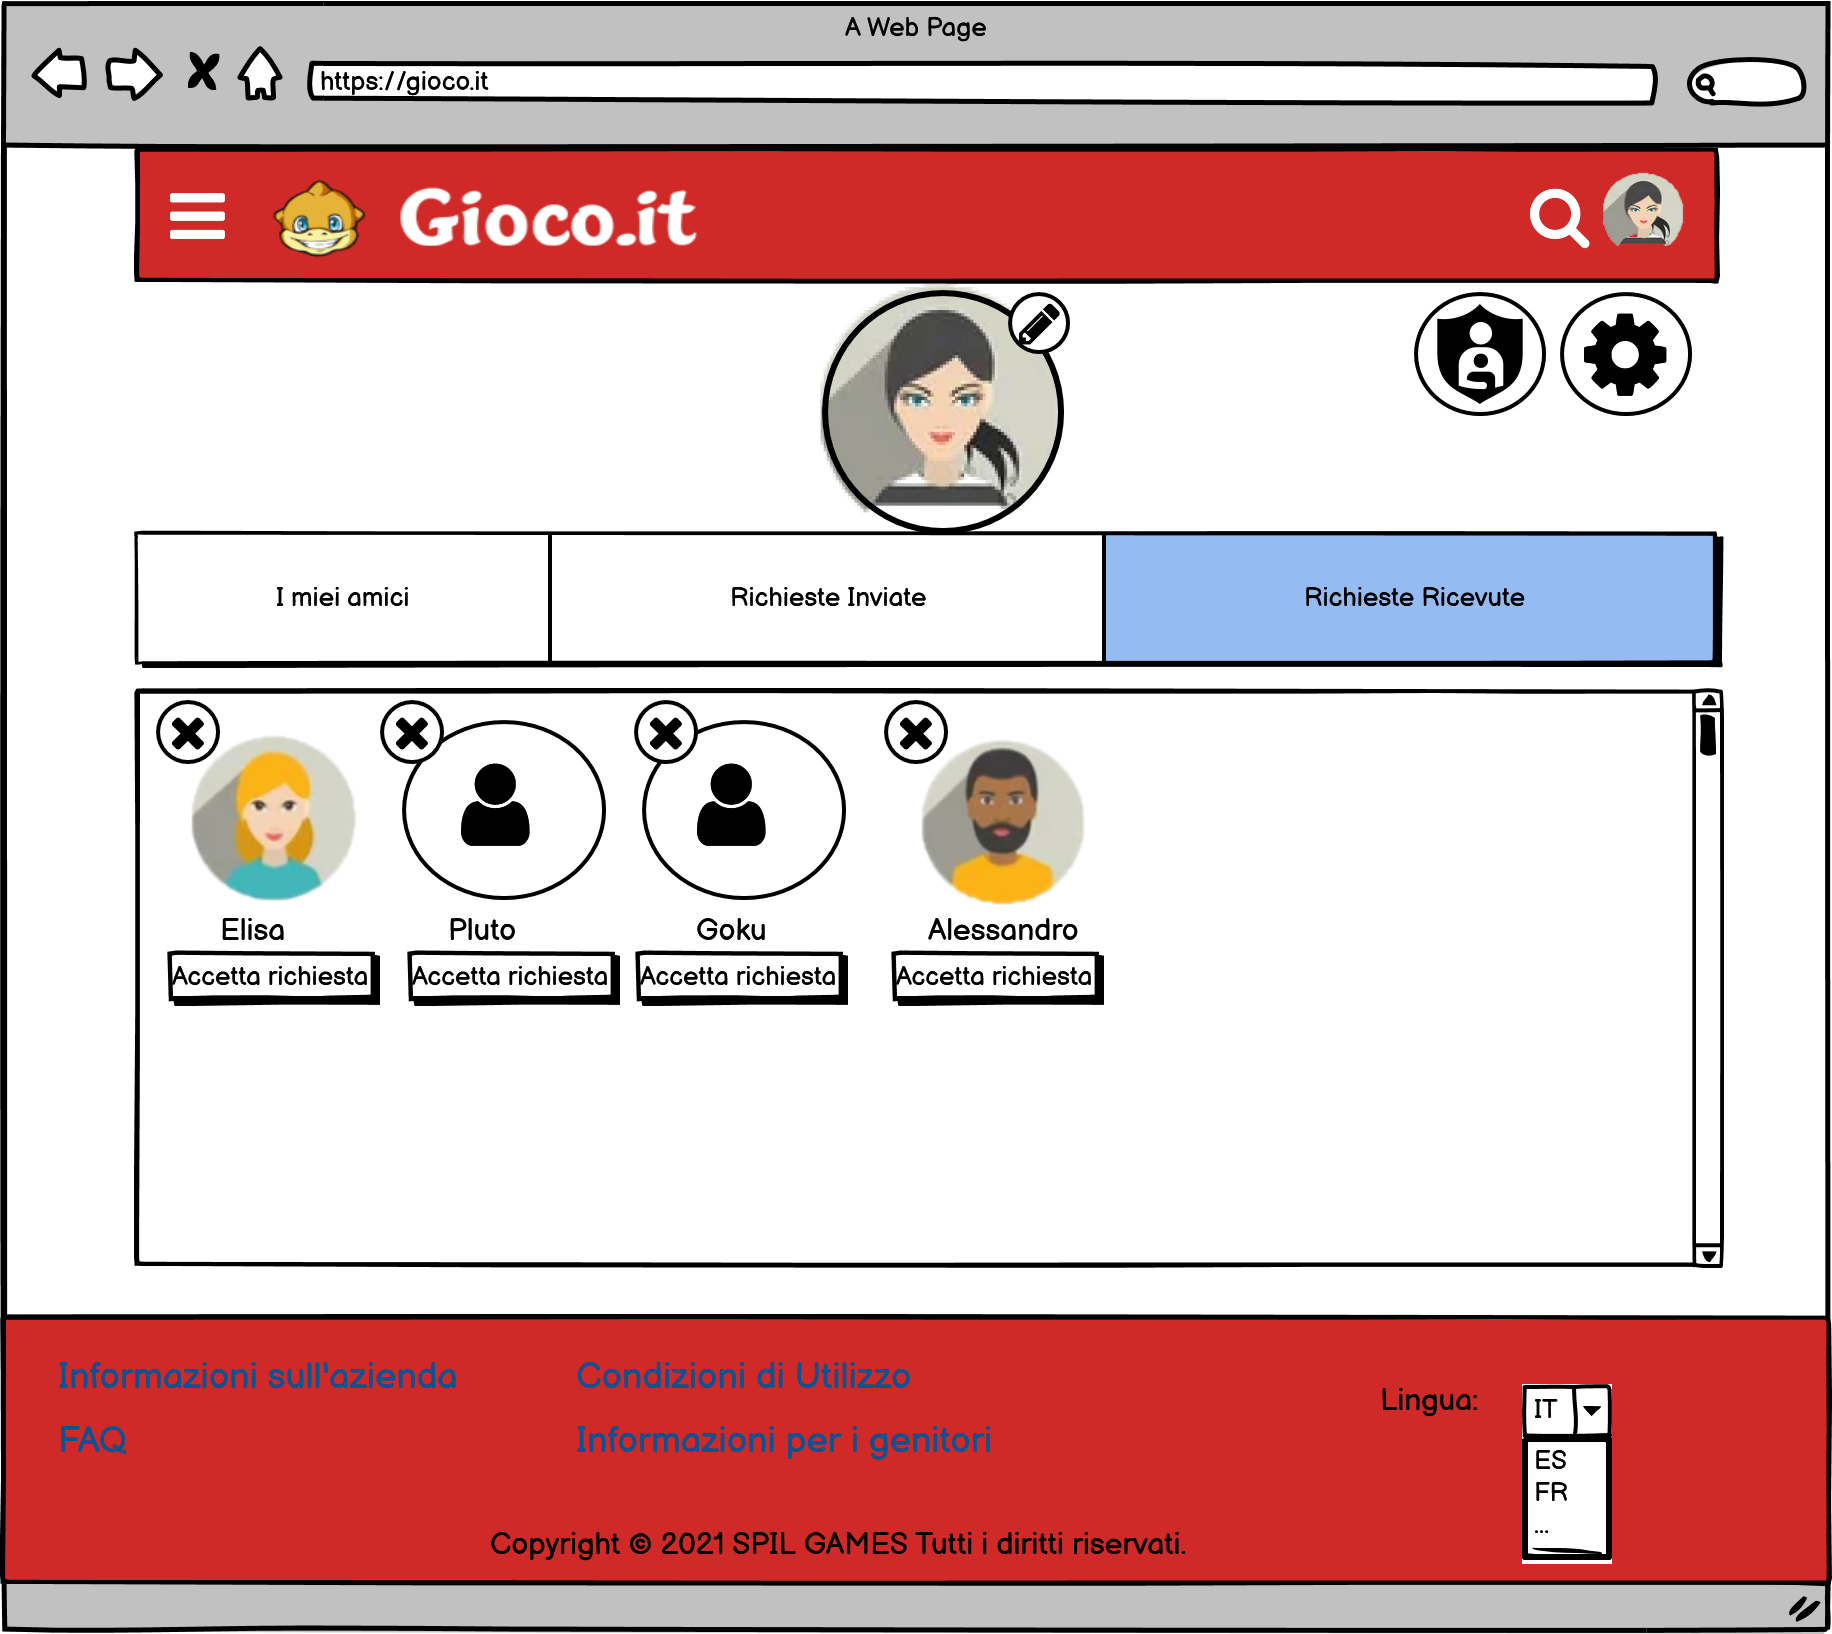
\includegraphics[width=8cm]{WAmici3.png}
        \end{minipage}
    \end{figure}

    Nella seconda tab è possibile visualizzare le richieste d'amicizia inviate e decidere se annullarle, mentre nella terza è possibile visualizzare quelle ricevute e decidere se accettarle.

    \subsubsection{Sotto sezione 4}
    In questa sotto sezione si possono visualizzare le card degli ultimi giochi inseriti tra i preferiti. Nel caso volessimo visualizzarli tutti basterà fare click sul pulsante "Mostra Tutti" ed esso ci condurrà ad una nuova schermata:
    \begin{figure}[H]
        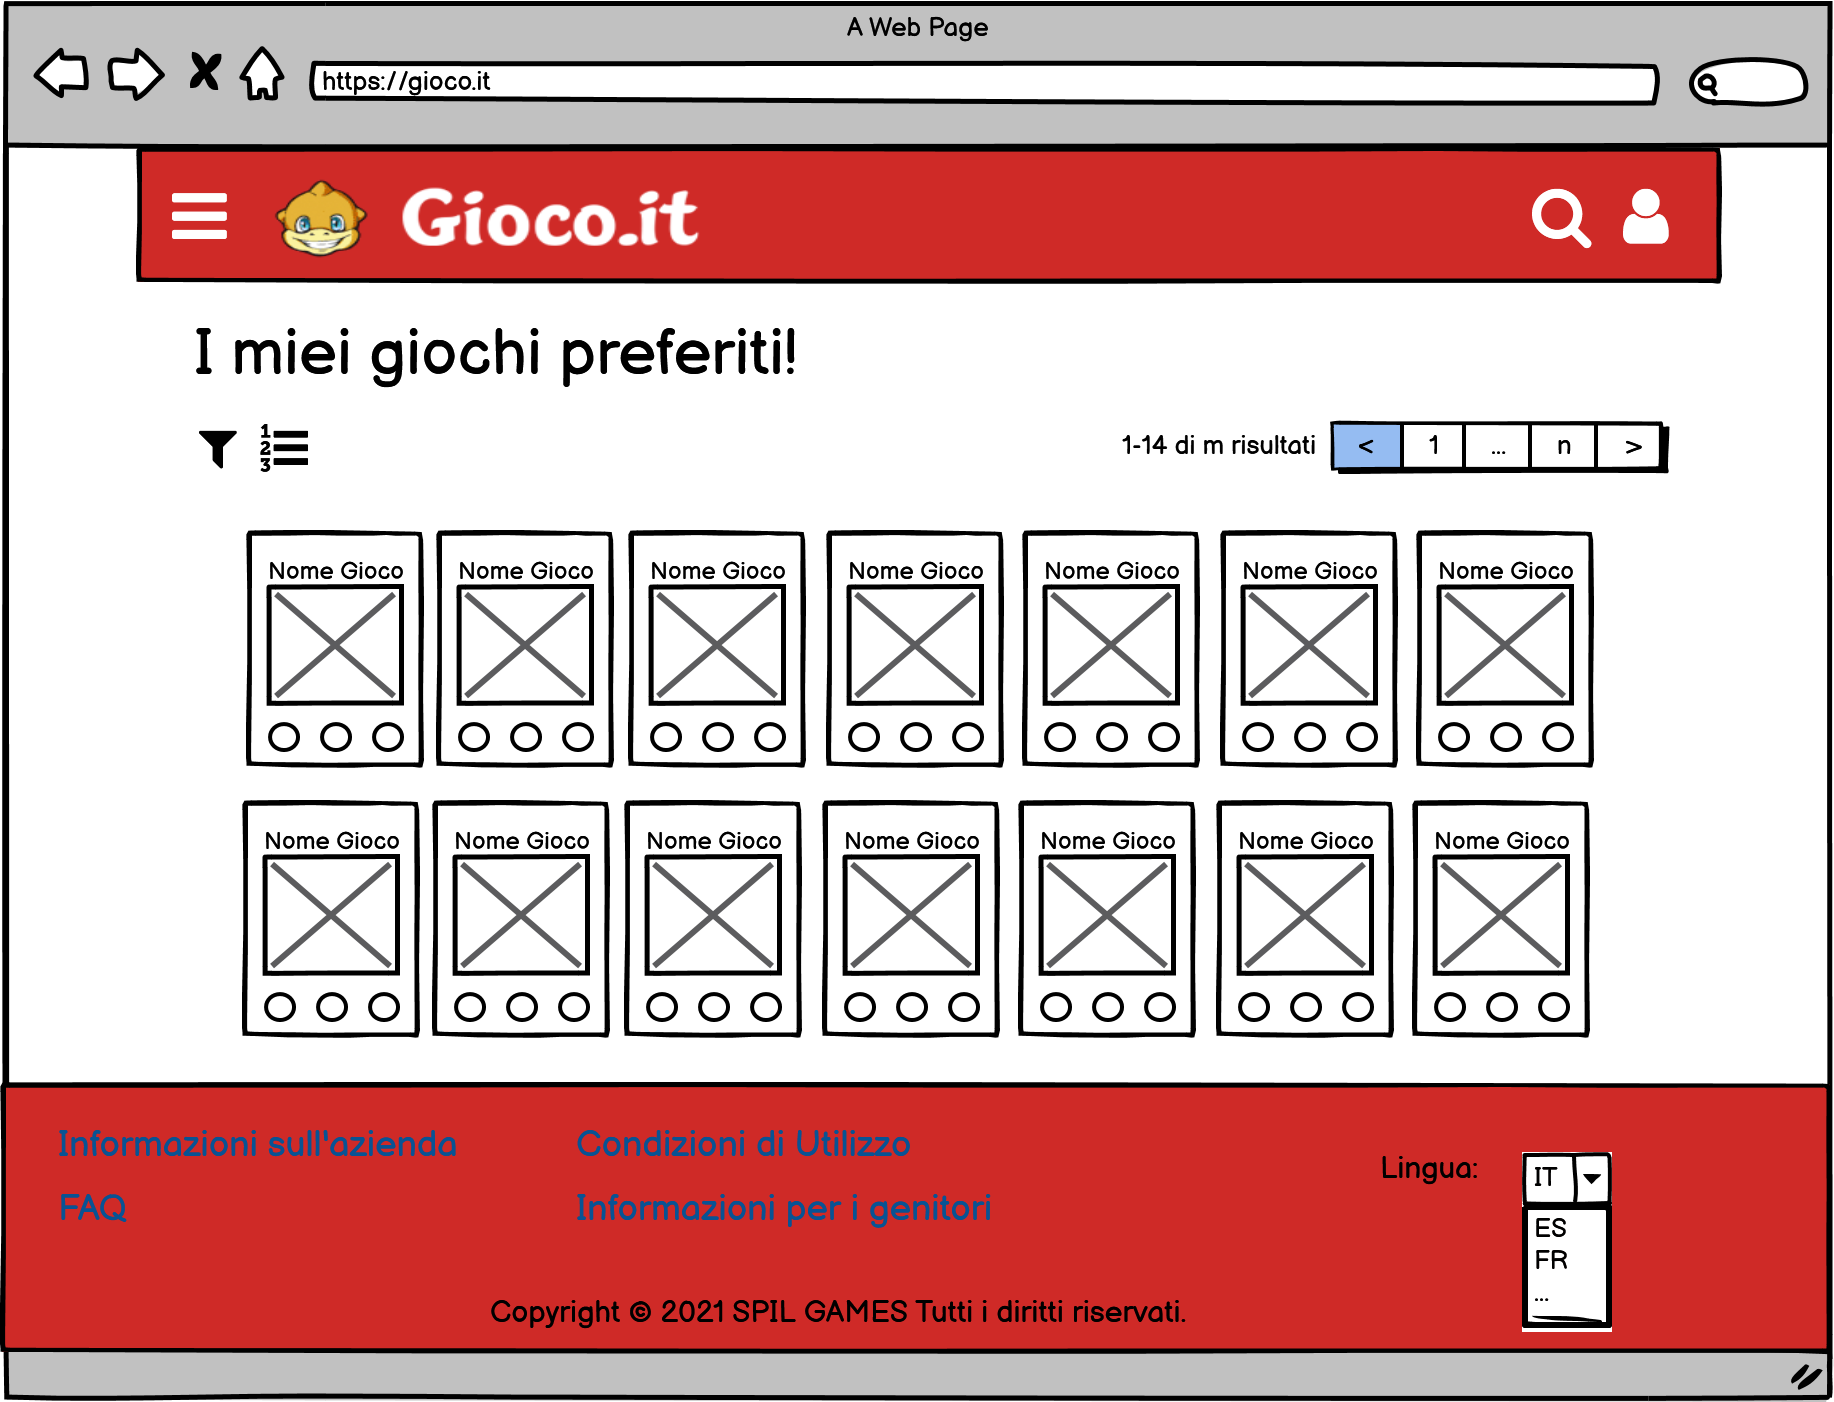
\includegraphics[width=10cm]{WPreferiti.png}
        \centering
    \end{figure}
    Qui sarà possibile scorrerli tutti, visualizzarne solo alcuni in base a dei filtri, giocarci e levarli dai preferiti.

    \subsection{Parental Control}
    \label{section: parental control}

\end{document}